\chapter {Thực nghiệm và đánh giá mô hình}

Trong đề tài này, công việc chính là huấn luyện một tác nhân có
khả năng tư vấn sản phẩm thời gian dùng mô hình học tăng cường.
Để hiện thực mô hình này có khả năng sử dụng trong thực tế, đề tài
còn thực hiện một ứng dụng Chatbot đơn giản, có ngõ nhập bằng
ngôn ngữ tự nhiên cho người dùng thông thường và nơi nhập
\textit{user action} (hành động người dùng) ở dạng khung ngữ nghĩa
nhằm kiểm tra khả năng hoạt động của tác nhân, bỏ qua các lỗi sai
khi nhận dạng ngôn ngữ tự nhiên. Vì vậy, ở phần này thực hiện
kiểm thử và đánh giá cho cả mô hình lẫn ứng dụng Chatbot.

\section{Đánh giá mô hình}

\subsection{Đánh giá giải thuật học tăng cường}
Để tác nhân có thể hoạt động được ngay sau khi quá trình huấn luyện
kết thúc, nó phải được \enquote{học}, \enquote{khám phá} và tối đa hóa
phần thưởng nhận được. Đánh giá thuật toán học tăng cường này bằng cách
chỉ ra nó nhận được phần thưởng bao nhiêu trong quá trình được huấn luyện.

Mô hình được huấn luyện với các thông số như mô tả trong mục \ref{subsec:agent}.
Số lượt hội thoại trong giai đoạn huấn luyện là 40000.

Hình \ref{fig:rewardtrain} thể hiện hiệu suất của thuật toán
học tăng cường, một biểu đồ đường cong huấn luyện biểu diễn
phần thưởng mà tác nhân nhận được khi kết thúc cuộc hội thoại.
Vì số lượt câu thoại cho phép lớn nhất là 20, nên phần thưởng
nhỏ nhất nhận được cho hội thoại thất bại là -40, phần thưởng
lớn nhất nhận được cho hội thoại thành công là 40 (không bao giờ
đạt được phần thưởng lớn nhất vì phần thưởng luôn giảm qua
từng lượt câu thoại). Phần thưởng được ghi lại sau 100 lượt
hội thoại và tính giá trị trung bình.

\begin{figure}[ht!]
    \centering
    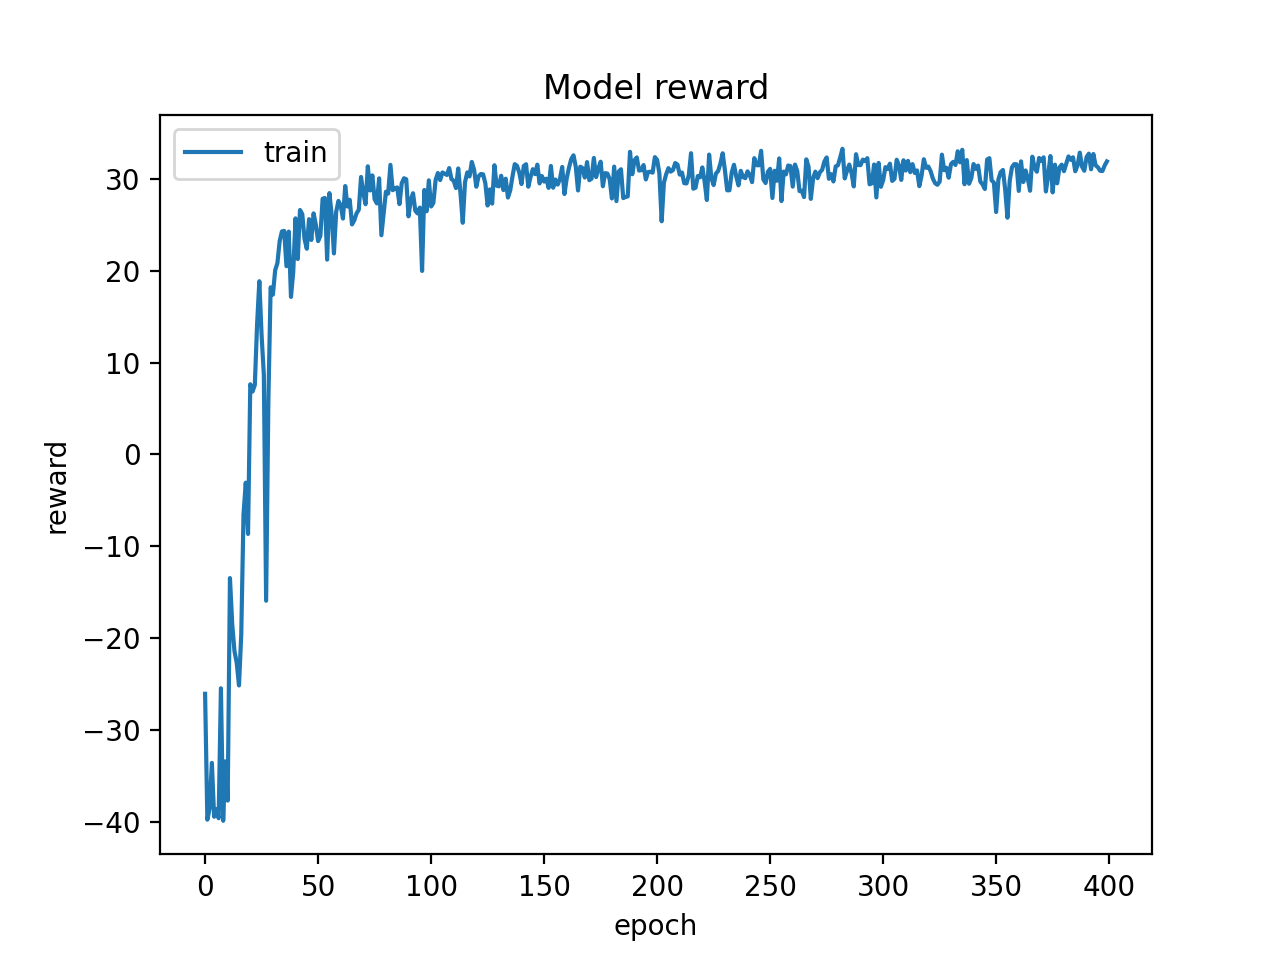
\includegraphics[scale=0.95]{thesis/chatbot/ketqua/img/rewardtrain.png}
    \caption{Biểu đồ đường cong huấn luyện cho phần thưởng}
    \label{fig:rewardtrain}
\end{figure}

\subsubsection{Nhận xét}
Với kết quả biểu diễn ở hình \ref{fig:rewardtrain}, ta thấy:

\begin{itemize}
    \item Giai đoạn đầu, phần thưởng nhận được là cực thấp.
    Vì thời gian đầu, tác nhân cần được khám phá thị trường
    một cách tổng quát nhất.
    \item Tuy nhiên, để phần thưởng nhận được trở nên tích cực,
    nó chỉ mất khoảng 5000 đến 10000 lượt hội thoại.
    \item Độ dốc đường cong ở các epoch cuối là thấp, phần thưởng
    nhận được khá ổn định trong giai đoạn cuối của huấn luyện.
    Chứng tỏ, huấn luyện được mô hình có chính sách (policy) ổn định.
    \item Kết quả cuối huấn luyện của mô hình khá tốt.
    Phần thưởng giao động trên 30 điểm.
\end{itemize}

% Có ba số liệu thống kê của biểu đồ này quan trọng:
% • Độ dốc tiệm cận cho thấy chính sách tốt như thế nào sau khi thuật toán đã ổn định.
% • Mức tối thiểu của đường cong cho thấy phần thưởng phải được hy sinh trước khi nó bắt đầu cải thiện.
% • Việc vượt qua số 0 cho thấy phải mất bao lâu cho đến khi thuật toán thu hồi được chi phí học tập của nó.

Ngoài ra, ta còn có một biểu đồ đường cong huấn luyện biểu diễn
tỉ lệ thành công của hội thoại như hình \ref{fig:successtrain}.
Tỉ lệ thành công được tính của 100 lượt hội thoại.

\begin{figure}[ht!]
    \centering
    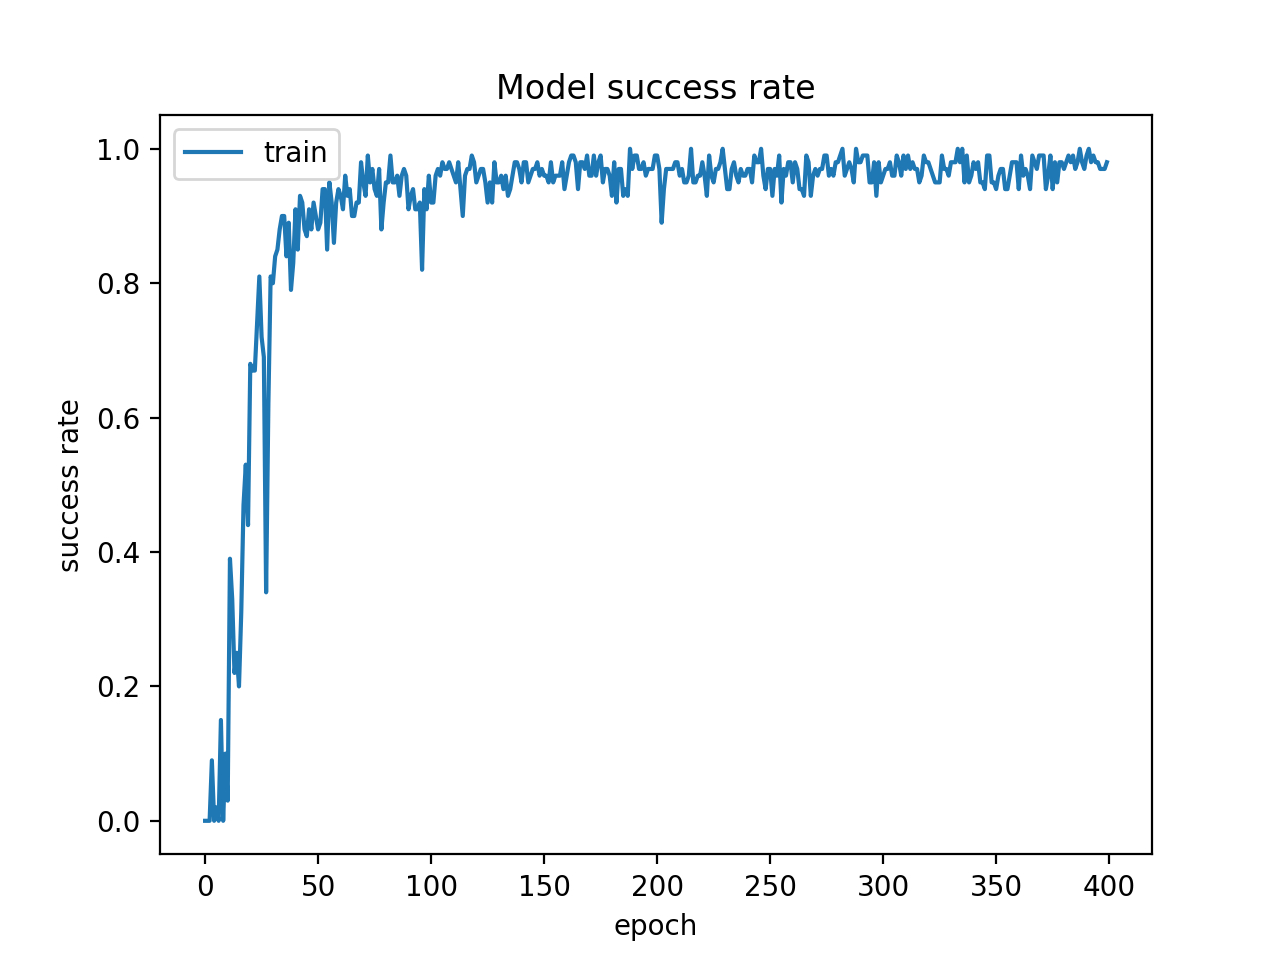
\includegraphics[scale=0.95]{thesis/chatbot/ketqua/img/successtrain.png}
    \caption{Biểu đồ đường cong huấn luyện cho tỉ lệ thành công}
    \label{fig:successtrain}
\end{figure}

\subsubsection{Nhận xét}
Với kết quả biểu diễn ở hình \ref{fig:successtrain}, ta thấy:

\begin{itemize}
    \item Giai đoạn đầu, tỉ lệ thành công là cực thấp. Tương đương
    với phần thưởng nhận được thấp như mô tả ở hình \ref{fig:rewardtrain}.
    \item Tỉ lệ thành công cũng trở nên tốt hơn sau 5000 đến
    10000 lượt hội thoại.
    \item Độ dốc đường cong ở các epoch cuối là thấp, tỉ lệ
    thành công khá ổn định trong giai đoạn cuối của huấn luyện.
    \item Kết quả cuối huấn luyện của mô hình khá tốt.
    Tỉ lệ thành công giao động từ 0.97 đến 1.
\end{itemize}

\subsection{Kiểm thử mô hình sử dụng bộ mô phỏng người dùng}
Như đã trình bày ở mục \ref{sec:usersim}, \textit{User Simulator} là
bộ mô phỏng người dùng thật để tương tác với tác nhân. Sau khi
huấn luyện, ta cũng có thể sử dụng nó để đánh giá mô hình. Việc dùng
bộ mô phỏng người dùng cho việc đánh giá sẽ giảm thiểu thời gian và
công sức rất nhiều so với người dùng thật. Ngoài ra, bằng cách chạy
tự động và với tập dữ liệu mục tiêu người dùng, chúng ta đánh giá
được mô hình với nhiều loại kịch bản khác nhau.

Hệ thống để đánh giá mô hình tương tự như quá trình huấn luyện.
Với bộ mô phỏng người dùng, ta chỉ đánh giá với tiêu chí là cuộc
hội thoại có thành công hay không, cụ thể được mô tả như sau:

\subsubsection{Tiêu chí đánh giá}
Cuộc hội thoại kết thúc thành công khi:

\begin{itemize}
    \item Các thông tin mà tác nhân cung cấp không xung đột với
    các ràng buộc mà người dùng cung cấp.
    \item Hoàn thành đủ mục tiêu của người dùng, các thông tin mà
    người dùng yêu cầu được cung cấp đầy đủ bởi tác nhân.
    \item Tác nhân tìm thấy sản phẩm thỏa mãn mọi yêu cầu của
    người dùng. Mục tiêu cuối cùng của Chatbot này chốt được đơn hàng
    cho người dùng nên trong trường hợp tác nhân tìm thấy thông tin
    sản phẩm nhưng bị từ chối bởi người dùng vẫn tính là không thành công.
\end{itemize}

\subsubsection{Kết quả}
Sử dụng tập mục tiêu người dùng (User Goal) như mô tả ở mục
\ref{subsec:usergoal}, sau 10000 cuộc hội thoại diễn ra, ta đạt được
xác suất \textbf{96\%} cuộc hội thoại thành công.

\subsubsection{Nhận xét}
Với kết quả 96\% cuộc hội thoại thành công, tác nhân đã gần như lúc nào
cũng hoàn thành được nhu cầu của người dùng. Sau khi phân tích cụ thể
các trường hợp không thành công, đa phần đến từ việc tư vấn kích cỡ
sản phẩm phù hợp cho người dùng. Nguyên nhân do dữ liệu về kích cỡ
cơ thể chưa đủ phong phú để tìm được kích cỡ phù hợp, và một phần do
số đo cơ thể người dùng thực sự không phù hợp cho các sản phẩm mà
cửa hàng kinh doanh.

\subsection{Đánh giá từ người dùng thực}
Để nhận đánh giá từ người dùng một cách nhanh chóng và rõ ràng, trong
luận án này, xây dựng một bộ các câu hội thoại/ đoạn hội thoại, gửi
cho một số người dùng thực tế để đánh giá. Ngoài ra, thực hiện so sánh
với một ứng dụng Chatbot tư vấn tương tự khác. Chatbot này không
huấn luyện mô hình mà chỉ thực hiện theo một bộ luật định sẵn (Chatbot
rule-based). Việc này nhằm mục đích so sánh Chatbot huấn luyện theo
mô hình học tăng cường đạt được mục tiêu ứng dụng thực tế nhất định.

\subsubsection{Tiêu chí đánh giá}
Các tiêu chí đánh giá cho các câu thoại bao gồm:

\begin{itemize}
    \item Thỏa mãn yêu cầu người dùng đưa ra
    \item Tính hợp lý, thiết thực của các câu yêu cầu từ tác nhân
    \item Tính tự nhiên, dễ trả lời của các câu yêu cầu từ tác nhân
    \item Tính thiết thực, hữu ích của các thông tin mà tác nhân cung cấp
    \item Tính chính xác của các thông tin mà tác nhân cung cấp
\end{itemize}

Các tiêu chí đánh giá cho toàn bộ hội thoại bao gồm:

\begin{itemize}
    \item Mức độ đáp ứng nhu cầu tư vấn sản phẩm nói chung
    \item Mức độ giao tiếp tự nhiên trong suốt cuộc hội thoại
    \item Đánh giá tổng quan của người dùng
\end{itemize}

Toàn bộ các tiêu chí này sẽ được đánh giá thêm một cột rằng nó có
tốt hơn so với \textit{Chatbot rule-based} hay không.

\subsubsection{Nội dung đánh giá}
Các câu thoại tạo ra để mang đi đánh giá nên thể hiện tất cả các
trường hợp khi người dùng tham dự vào hội thoại. Cụ thể:

Nội dung đánh giá cho các câu thoại thông thường:

\begin{itemize}
    \item Chào hỏi với tác nhân gồm:
    \begin{itemize}
        \item Chào hỏi khi bắt đầu cuộc hội thoại
        \item Chào hỏi ở giữa cuộc hội thoại
        \item Chào hỏi khi kết thúc cuộc hội thoại
        \item Chào hỏi nhiều lần
    \end{itemize}
    \item Cám ơn/tạm biệt với tác nhân gồm:
    \begin{itemize}
        \item Khách hàng cám ơn shop sau khi xác nhận đặt hàng, được
        tư vấn sản phẩm
        \item Khách hàng cám ơn shop sau khi nhận được thông tin
        sản phẩm hữu ích
        \item Khách hàng cám ơn ở những trường hợp không liên quan khác
        \item Cám ơn nhiều lần
    \end{itemize}
    \item Khác: Khách hàng hỏi các thông tin khác không liên quan tới
    tư vấn sản phẩm
\end{itemize}

Tiêu chí đánh giá cho các câu thoại thông thường:

\begin{itemize}
    \item Tính hợp lý: Không hợp lý, phải cải thiện -> Không hợp lý
    lắm, nhưng chấp nhận được -> Hợp lý
    \item Tính tự nhiên: Không tự nhiên, phải cải thiện -> Không
    tự nhiên lắm, nhưng chấp nhận được -> Tự nhiên
    \item Tính hợp lý/ Tính tự nhiên so với \textit{Chatbot rule-based}:
    Tệ hơn -> Như nhau -> Tốt hơn
\end{itemize}

Nội dung đánh giá cho các câu thoại tư vấn:

\begin{itemize}
    \item Yêu cầu cung cấp thông tin sản phẩm. Trường hợp có hàng và
    không có hàng gồm:
    \begin{itemize}
        \item Gửi tên sản phẩm, hỏi đơn giá
        \item Gửi tên sản phẩm, hỏi màu sản phẩm
        \item Gửi tên sản phẩm, hỏi chất liệu sản phẩm
        \item Gửi tên sản phẩm, hỏi kích cỡ sản phẩm
        \item Gửi tên sản phẩm, kích cỡ, hỏi đơn giá
        \item Gửi tên sản phẩm, màu, hỏi đơn giá
        \item Gửi tên sản phẩm, kích cỡ, hỏi màu sản phẩm
        \item Gửi tên sản phẩm, màu, hỏi chất liệu sản phẩm
        \item Gửi tên sản phẩm, kích cỡ, hỏi chất liệu sản phẩm
        \item Gửi tên sản phẩm, màu, hỏi kích cỡ sản phẩm
        \item Gửi tên sản phẩm, hỏi còn hàng hay không
        \item Gửi tên sản phẩm, màu, hỏi còn hàng hay không
        \item Gửi tên sản phẩm, kích cỡ, hỏi còn hàng hay không
        \item Gửi tên sản phẩm, màu, kích cỡ, hỏi còn hàng hay không
    \end{itemize}
    \item Tư vấn chọn kích cỡ:
    \begin{itemize}
        \item Chỉ gửi chiều cao
        \item Chỉ nhập cân nặng
        \item Chỉ gửi vòng eo
        \item Gửi chiều cao, cân nặng
        \item Gửi chiều cao, vòng eo
        \item Gửi vòng eo, cân nặng
        \item Gửi chiều cao, cân nặng, vòng eo. Trường hợp có
        kích cỡ phù hợp
        \item Gửi chiều cao, cân nặng, vòng eo. Trường hợp không có
        kích cỡ phù hợp
    \end{itemize}
    \item Đặt hàng:
    \begin{itemize}
        \item Chỉ gửi tên sản phẩm
        \item Chỉ gửi màu sản phẩm
        \item Chỉ gửi kích cỡ sản phẩm
        \item Chỉ gửi số lượng sản phẩm
        \item Gửi màu, số lượng sản phẩm
        \item Gửi màu, kích cỡ sản phẩm
        \item Gửi kích cỡ, số lượng sản phẩm
        \item Gửi tên sản phẩm, màu
        \item Gửi tên sản phẩm, kích cỡ
        \item Gửi tên sản phẩm, số lượng
        \item Gửi tên sản phẩm, màu, kích cỡ
        \item Gửi tên sản phẩm, màu, số lượng
        \item Gửi tên sản phẩm, kích cỡ, số lượng
        \item Gửi tên sản phẩm, màu, kích cỡ, số lượng
    \end{itemize}
\end{itemize}

Tiêu chí đánh giá cho các câu thoại tư vấn:

\begin{itemize}
    \item Thỏa mãn yêu cầu người dùng đưa ra: Không thỏa mãn ->
    Chấp nhận được -> Thỏa mãn
    \item Tính hợp lý, thiết thực: Không hợp lý, phải cải thiện ->
    Không hợp lý lắm, nhưng chấp nhận được -> Hợp lý
    \item Tính tự nhiên, dễ trả lời: Không tự nhiên, phải cải thiện
    -> Không tự nhiên lắm, nhưng chấp nhận được -> Tự nhiên
    \item Tính thiết thực, hữu ích: Không thiết thực -> Chấp nhận
    được -> Thiết thực
    \item Tính chính xác: Không chính xác -> Chấp nhận được ->
    Chính xác
    \item So sánh với \textit{Chatbot rule-based} các tiêu chí trên:
    Tệ hơn -> Như nhau -> Tốt hơn
\end{itemize}

Nội dung đánh giá cho các hội thoại:

\begin{itemize}
    \item Hội thoại hỏi các thông tin của sản phẩm và chốt đơn hàng
    \item Hội thoại hỏi sản phẩm, mà cửa hàng không bán hoặc đã hết
    \item Hội thoại hỏi các thông tin của sản phẩm. Trường hợp các
    thông tin không tìm thấy sản phẩm phù hợp
    \item Tư vấn kích cỡ sản phẩm phù hợp với khách hàng
    \item Tư vấn kích cỡ sản phẩm phù hợp với khách hàng. Trường hợp
    không có kích cỡ thích hợp
    \item Thay đổi sản phẩm sau khi đặt hàng
\end{itemize}

Tiêu chí đánh giá cho các hội thoại:

\begin{itemize}
    \item Mức độ đáp ứng nhu cầu tư vấn sản phẩm nói chung: đánh giá
    5 mức độ từ chưa đáp ứng đến rất đầy đủ
    \item Mức độ giao tiếp tự nhiên: đánh giá 5 mức độ từ không
    tự nhiên đến rất tự nhiên
    \item Đánh giá tổng quan: với mức điểm từ một sao đến 5 sao
    \item So sánh với \textit{Chatbot rule-based} các tiêu chí trên:
    Tệ hơn -> Như nhau -> Tốt hơn
\end{itemize}

\subsubsection{Kết quả đánh giá}

\subsubsection{Tiêu chí thỏa mãn yêu cầu người dùng đưa ra}
Hình \ref{fig:tieuchi1} mô tả kết quả đánh giá của người dùng cho
tiêu chí thỏa mãn yêu cầu người dùng đưa ra khi Chatbot trả về kết quả.

\begin{figure}[ht!]
    \centering
    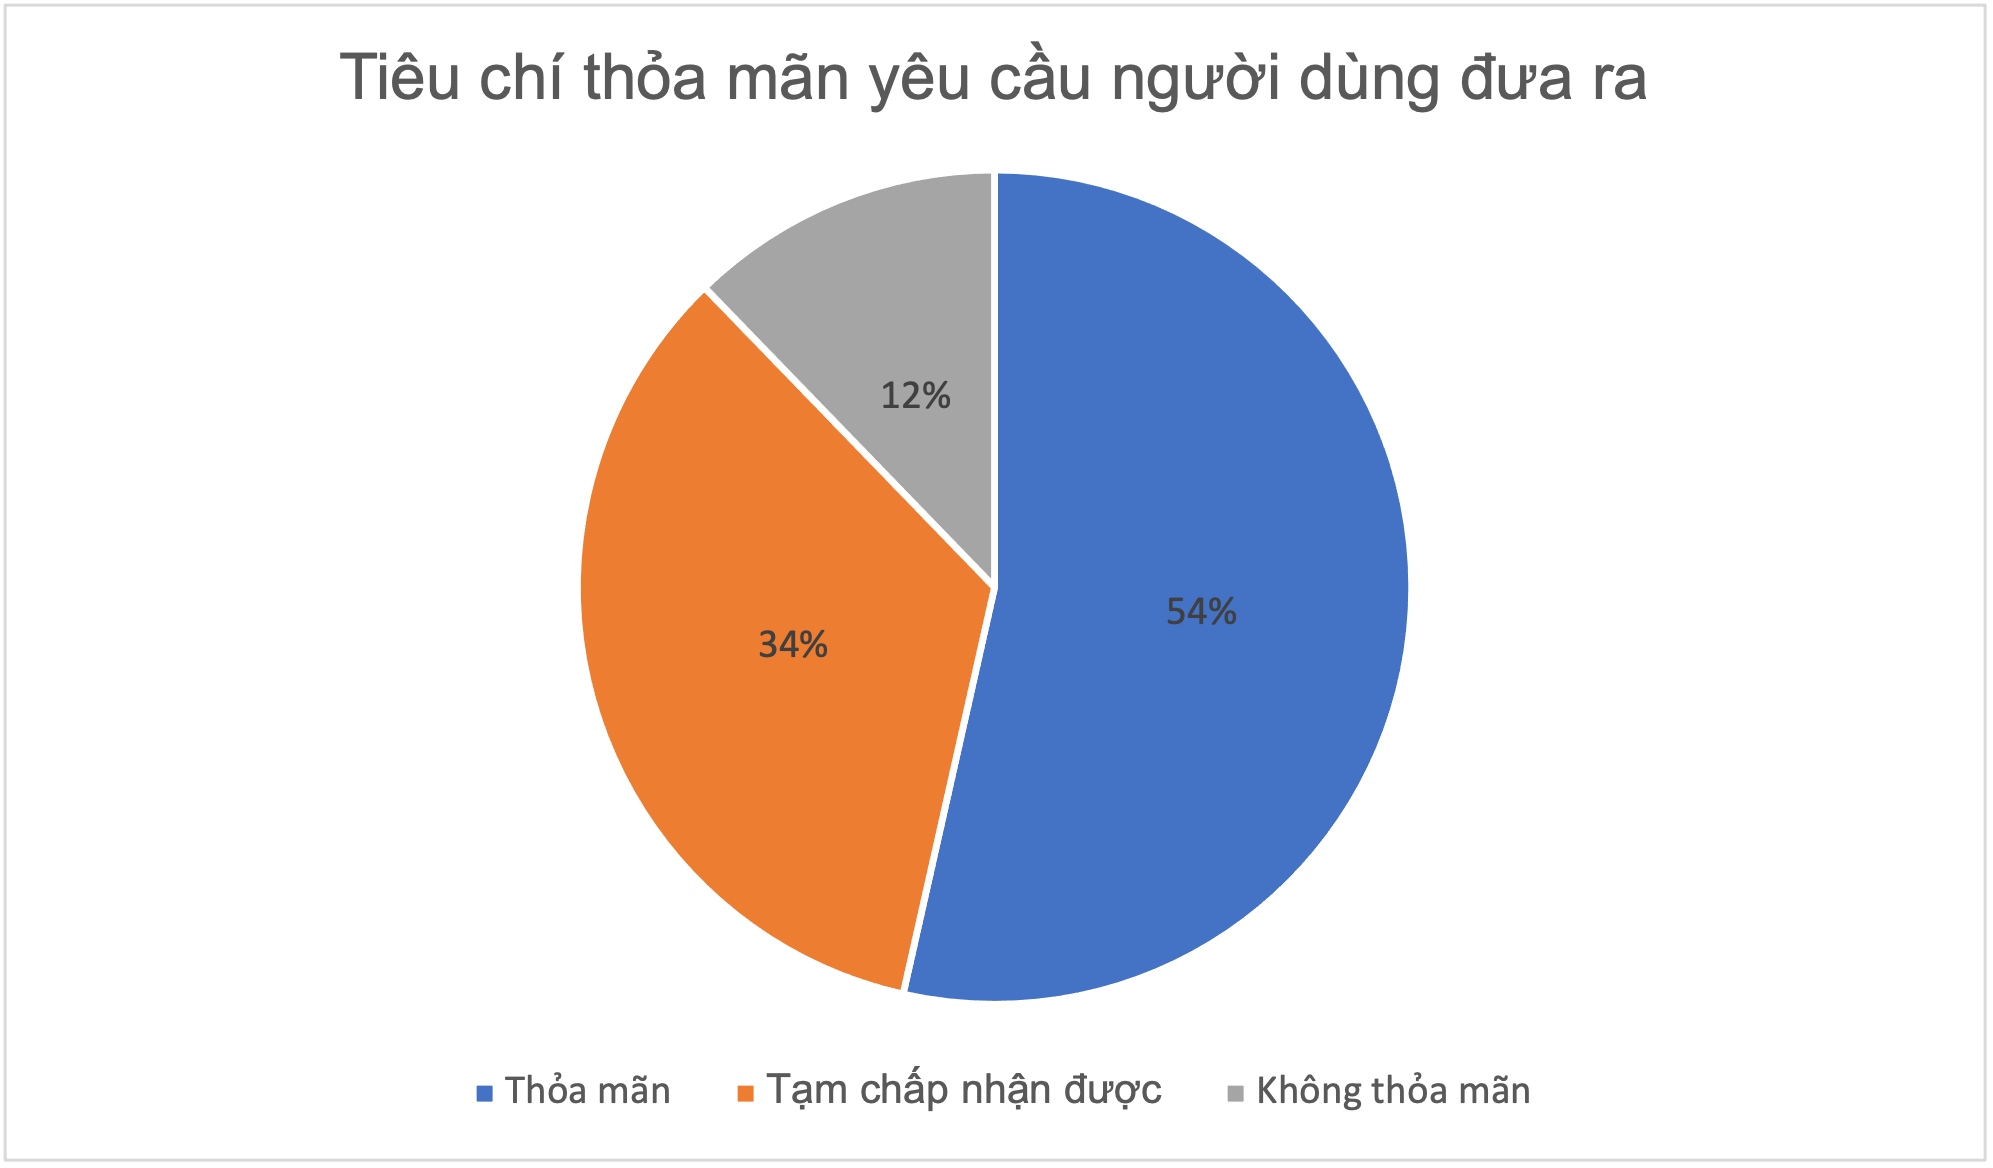
\includegraphics[scale=0.91]{thesis/chatbot/ketqua/img/tieuchi1.png}
    \caption{Kết quả đánh giá tiêu chí thỏa mãn yêu cầu người dùng}
    \label{fig:tieuchi1}
\end{figure}

\textbf{Nhận xét:}
Có 88\% nhận xét từ tạm chấp nhận được cho đến thỏa mãn hết các
yêu cầu. Trong đó hơn 50\% là thỏa mãn. Chỉ có 12\% nhận xét là không
thỏa mãn. Sau khi phân tích cụ thể các kết quả đánh giá không
thỏa mãn, nhận thấy các đánh giá này đa phần đến từ khi người dùng
yêu cầu một thông tin nào đó của sản phẩm không tồn tại trong cơ sở
dữ liệu (cửa hàng không bán hoặc hết hàng) và không cung cấp được
thông tin họ yêu cầu.

\subsubsection{So sánh với Chatbot rule-based}
Hình \ref{fig:tieuchi12} mô tả kết quả đánh giá của người dùng khi
so sánh tiêu chí thỏa mãn yêu cầu người dùng đưa ra với Chatbot
rule-based.

\begin{figure}[ht!]
    \centering
    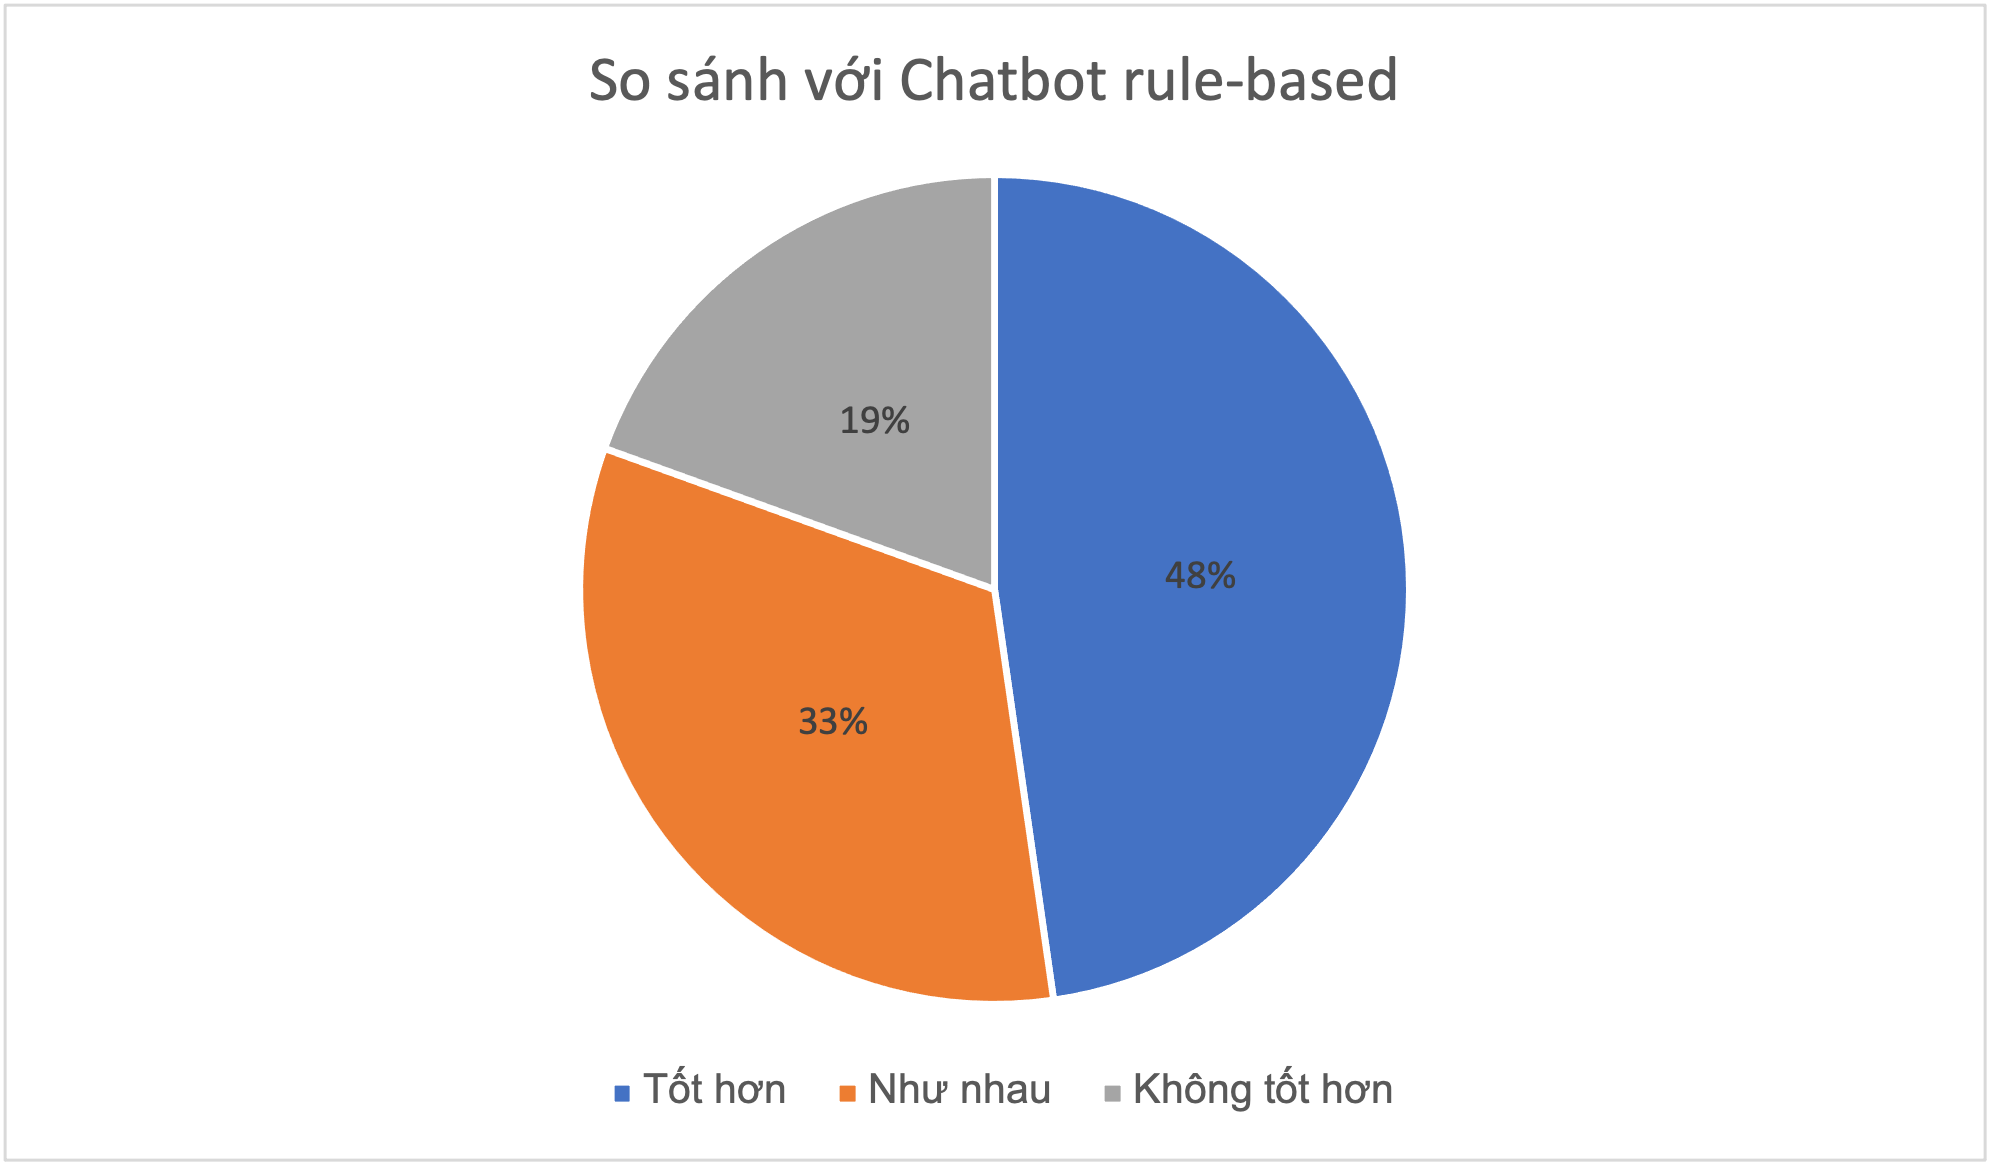
\includegraphics[scale=0.91]{thesis/chatbot/ketqua/img/tieuchi1_2.png}
    \caption{Kết quả so sánh với Chatbot rule-based}
    \label{fig:tieuchi12}
\end{figure}

\textbf{Nhận xét:}
Có hơn 80\% đánh giá là tốt hơn hoặc tương đương với Chatbot
rule-based. Có 19\% là không tốt hơn. Sau khi phân tích cụ thể các
kết quả đánh giá không tốt, nhận thấy Chatbot rule-based này sẽ
liệt kê tất cả thông tin của sản phẩm trong lượt đầu. Việc này
thỏa mãn một số người dùng tốt hơn Chatbot khi sử dụng học tăng cường.

\subsubsection{Tiêu chí về tính hợp lý, thiết thực của các câu
yêu cầu từ tác nhân}
Hình \ref{fig:tieuchi2} mô tả kết quả đánh giá của người dùng cho
tiêu chí tính hợp lý, thiết thực của các câu yêu cầu từ tác nhân.

\begin{figure}[ht!]
    \centering
    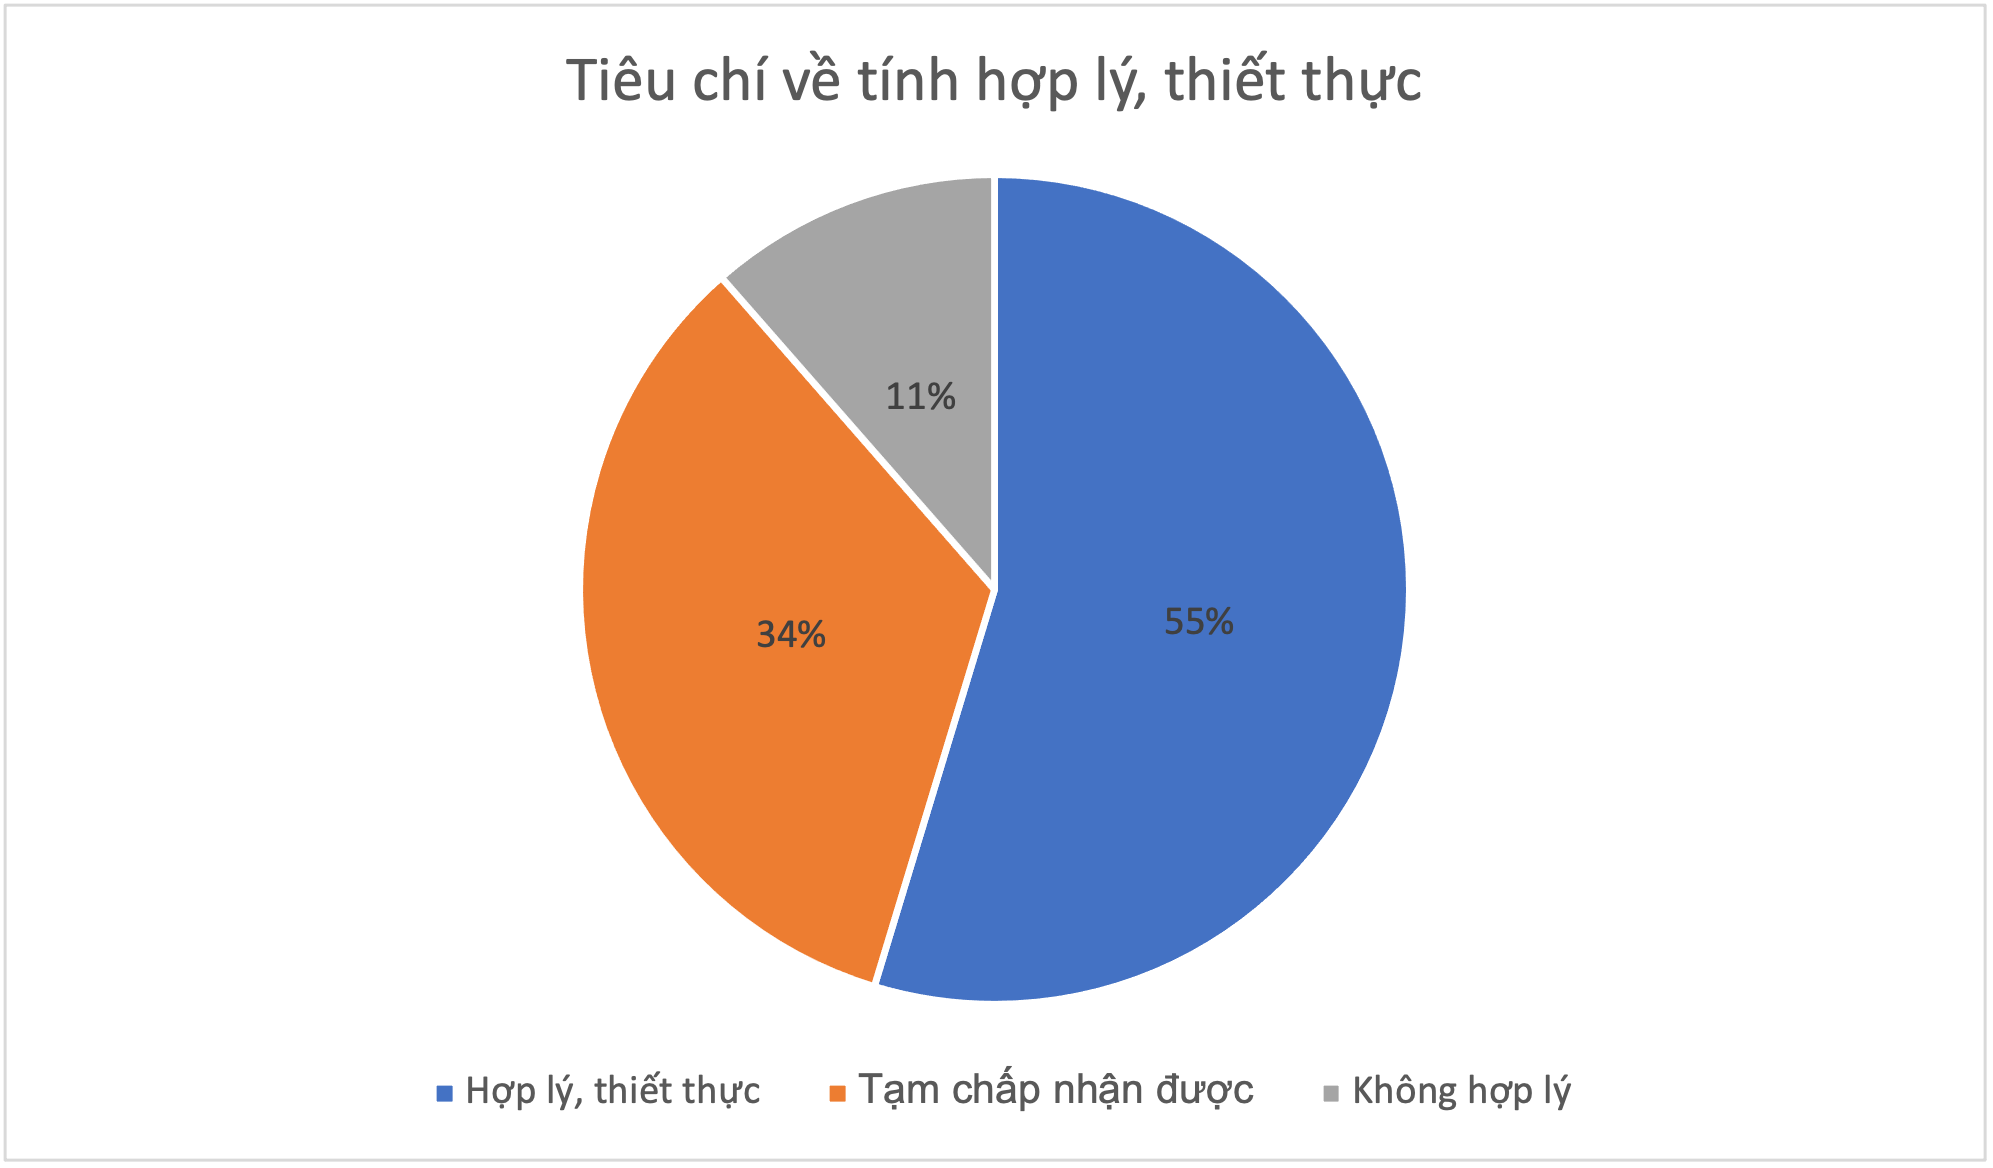
\includegraphics[scale=0.91]{thesis/chatbot/ketqua/img/tieuchi2.png}
    \caption{Kết quả đánh giá tiêu chí tính hợp lý, thiết thực}
    \label{fig:tieuchi2}
\end{figure}

\textbf{Nhận xét:}
Có gần 90\% nhận xét từ tạm chấp nhận được cho đến hợp lý. Trong đó
hơn 50\% là hợp lý. Chỉ có 11\% nhận xét là không hợp lý. Sau khi
phân tích cụ thể các kết quả đánh giá không hợp lý, nhận thấy các
đánh giá này đa phần đến từ khi người dùng yêu cầu một thông tin
nào đó của sản phẩm, họ mong muốn Chatbot mau chóng trả lời thông tin
mà họ cần thay vì phải trải qua một số các câu thoại yêu cầu khác
trước khi trả về kết quả.

\subsubsection{So sánh với Chatbot rule-based}
Hình \ref{fig:tieuchi22} mô tả kết quả đánh giá của người dùng khi
so sánh tiêu chí tính hợp lý, thiết thực với Chatbot rule-based.

\begin{figure}[ht!]
    \centering
    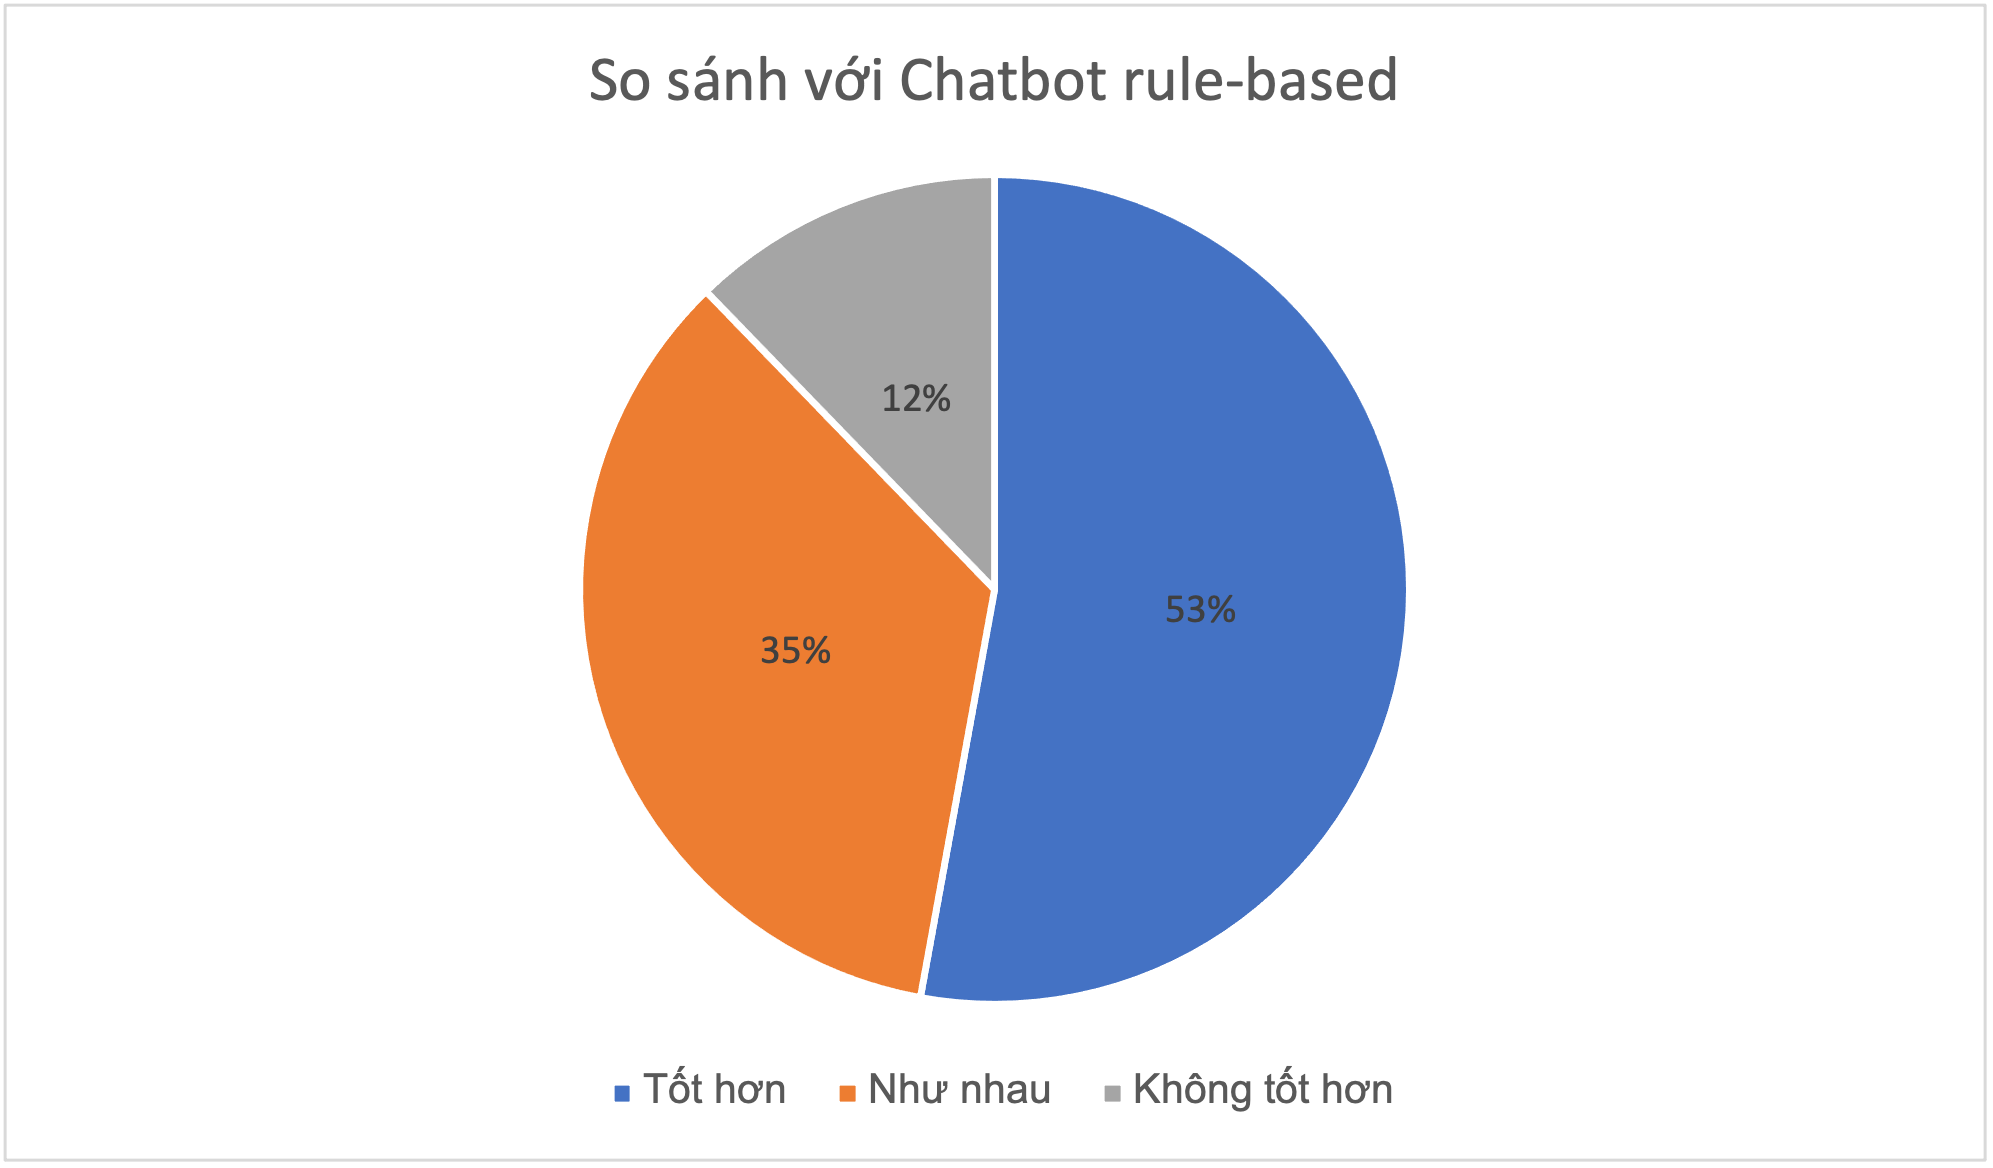
\includegraphics[scale=0.91]{thesis/chatbot/ketqua/img/tieuchi2_2.png}
    \caption{Kết quả so sánh với Chatbot rule-based}
    \label{fig:tieuchi22}
\end{figure}

\textbf{Nhận xét:}
Có gần 90\% đánh giá là tốt hơn hoặc tương đương với Chatbot
rule-based. Có 12\% là không tốt hơn. Sau khi phân tích cụ thể các
kết quả đánh giá không tốt, nhận thấy tương tự với lí do trên,
Chatbot rule-based này sẽ liệt kê tất cả thông tin của sản phẩm
trong lượt đầu. Việc này thỏa mãn một số người dùng tốt hơn Chatbot
khi sử dụng học tăng cường.

\subsubsection{Tiêu chí về tính tự nhiên, dễ trả lời của các câu
yêu cầu từ tác nhân}
Hình \ref{fig:tieuchi3} mô tả kết quả đánh giá của người dùng cho
tiêu chí tính tự nhiên, dễ trả lời của các câu yêu cầu từ tác nhân.

\begin{figure}[ht!]
    \centering
    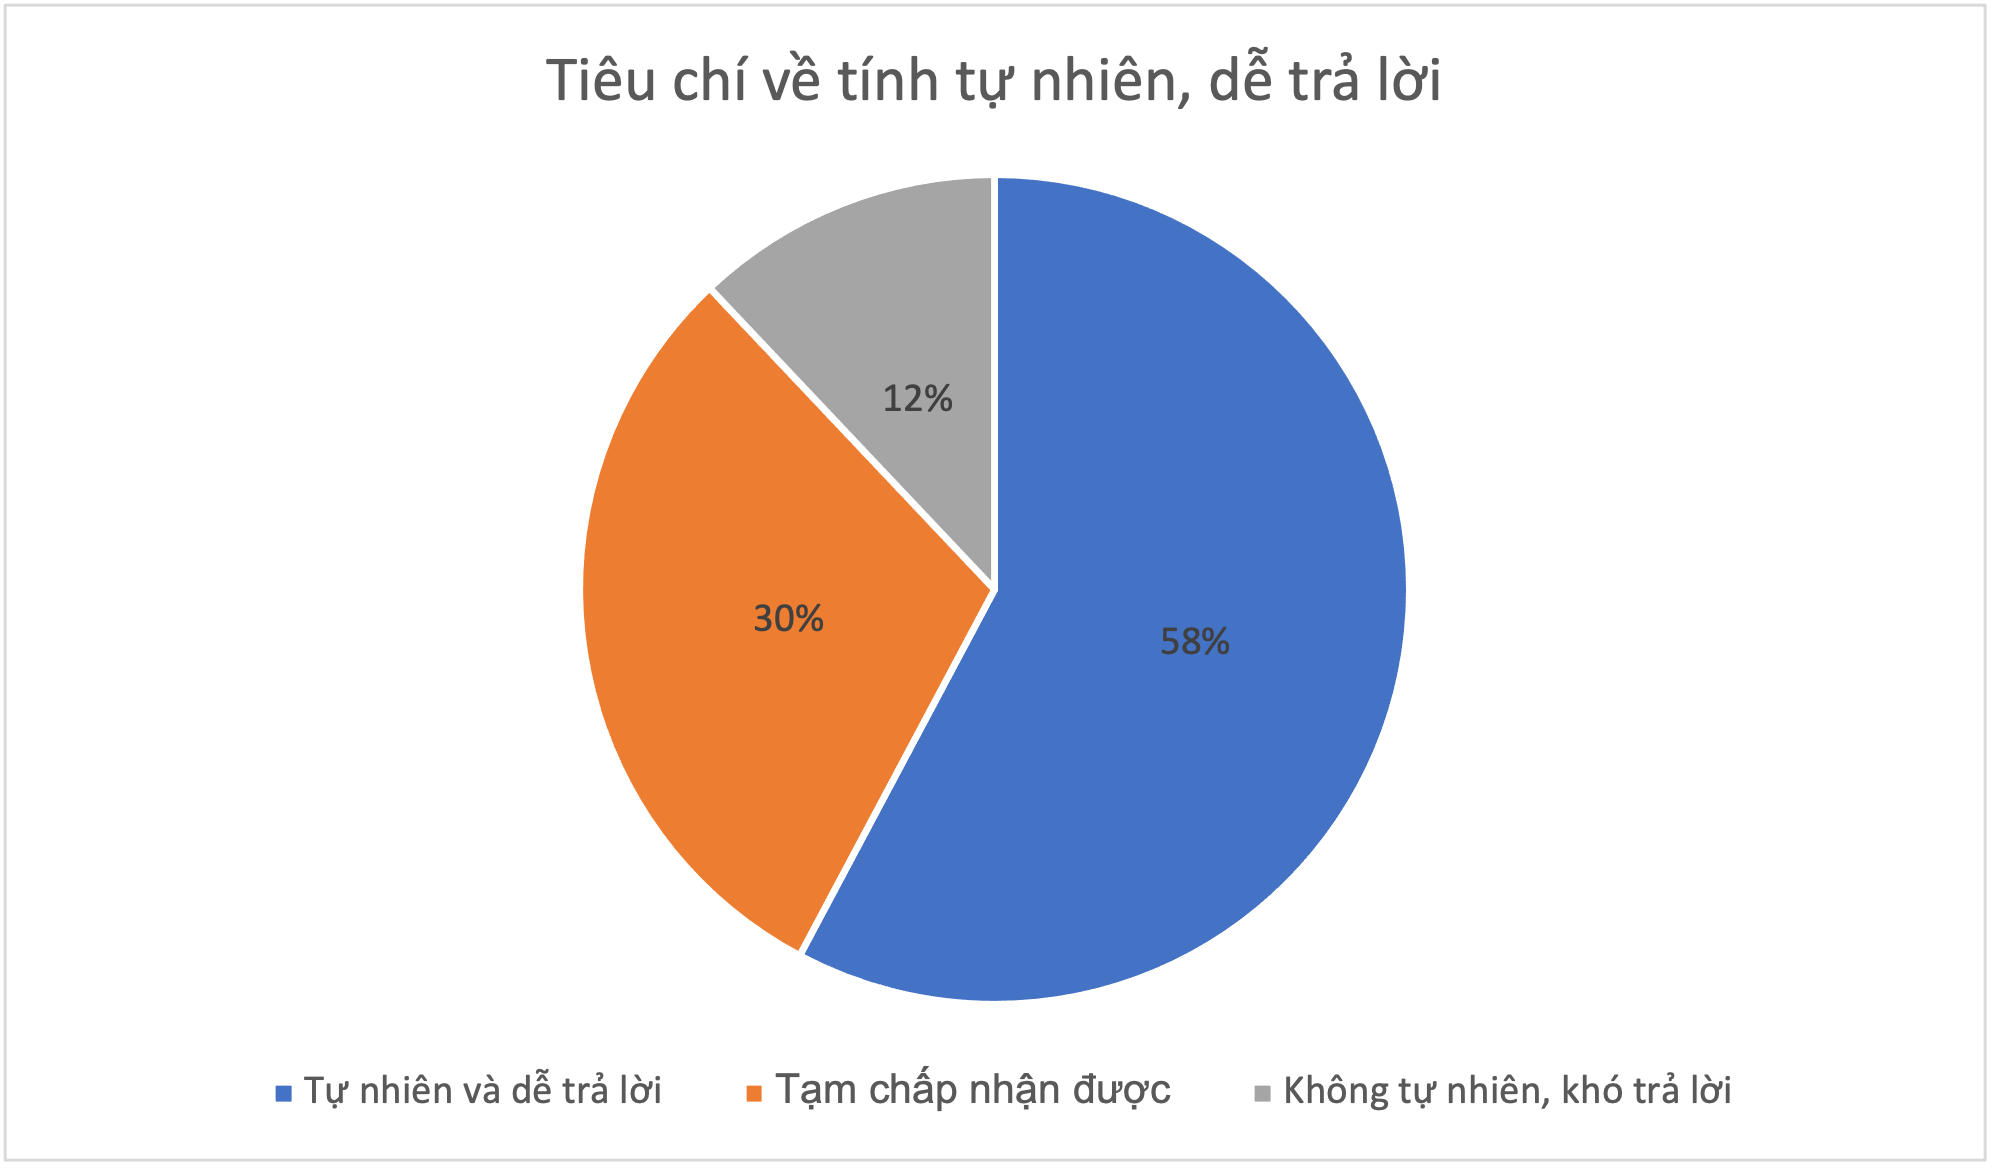
\includegraphics[scale=0.91]{thesis/chatbot/ketqua/img/tieuchi3.png}
    \caption{Kết quả đánh giá tiêu chí tính tự nhiên, dễ trả lời}
    \label{fig:tieuchi3}
\end{figure}

\textbf{Nhận xét:}
Có gần 90\% nhận xét từ tạm chấp nhận được cho đến tự nhiên. Trong đó
hơn 50\% là tự nhiên. Chỉ có 12\% nhận xét là không tự nhiên. Sau khi
phân tích cụ thể các kết quả đánh giá không tự nhiên, nhận thấy các
đánh giá này có thể đến từ bộ sinh phản hồi chưa phù hợp, dẫn tới các
câu gây khó hiểu hoặc hiểu nhầm.

\subsubsection{So sánh với Chatbot rule-based}
Hình \ref{fig:tieuchi32} mô tả kết quả đánh giá của người dùng khi
so sánh tiêu chí tính tự nhiên, dễ trả lời với Chatbot rule-based.

\begin{figure}[ht!]
    \centering
    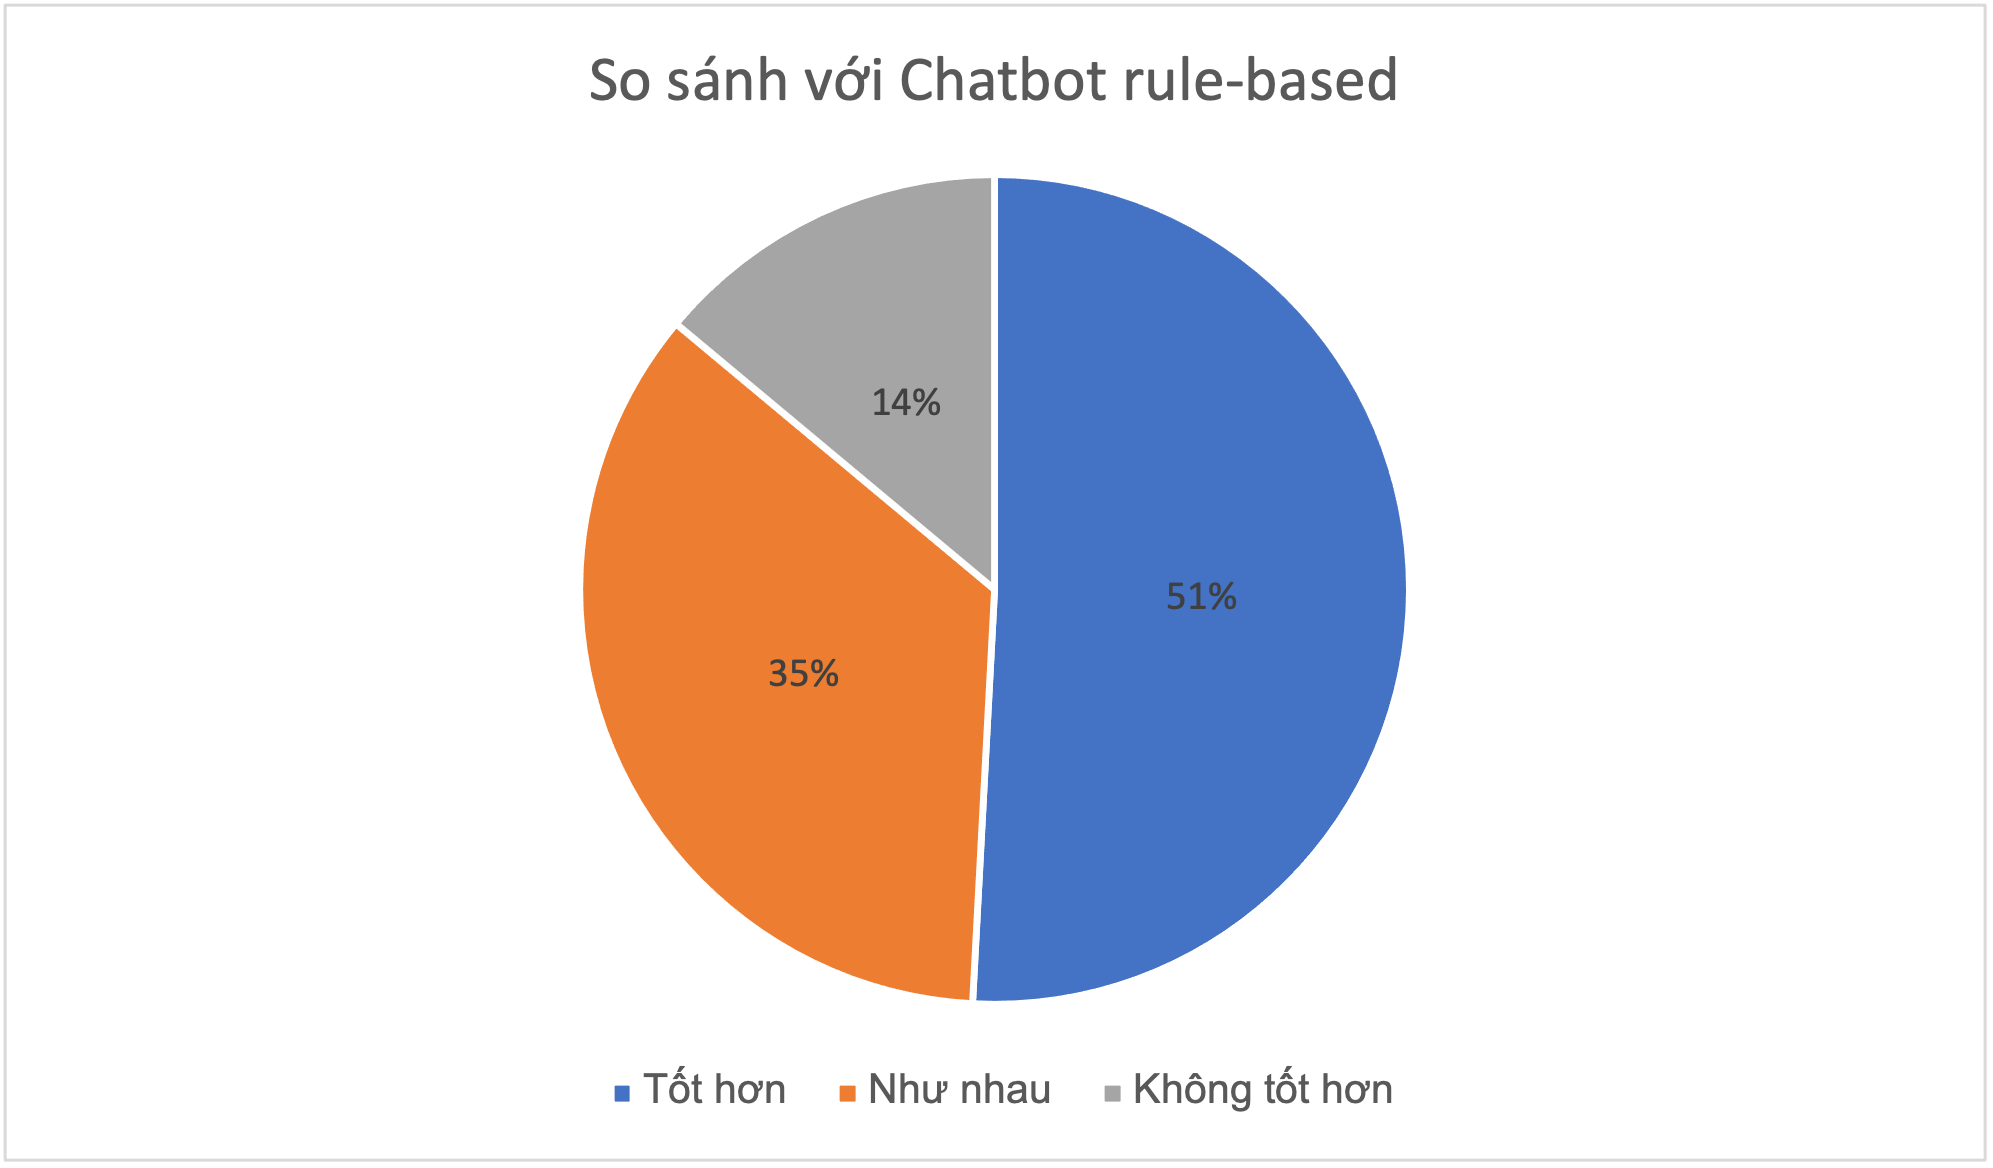
\includegraphics[scale=0.91]{thesis/chatbot/ketqua/img/tieuchi3_2.png}
    \caption{Kết quả so sánh với Chatbot rule-based}
    \label{fig:tieuchi32}
\end{figure}

\textbf{Nhận xét:}
Có gần 90\% đánh giá là tốt hơn hoặc tương đương với Chatbot rule-based.
Có 14\% là không tốt hơn. Sau khi phân tích cụ thể các kết quả đánh giá
không tốt, nhận thấy tương tự với lí do trên, Chatbot rule-based này sinh
câu phản hồi mà thỏa mãn một số người dùng tốt hơn Chatbot được
xây dựng trong đề tài.

\subsubsection{Tiêu chí về tính thiết thực, hữu ích của các thông tin
mà tác nhân cung cấp}
Hình \ref{fig:tieuchi4} mô tả kết quả đánh giá của người dùng cho tiêu chí
tính thiết thực, hữu ích của các thông tin mà tác nhân cung cấp.

\begin{figure}[ht!]
    \centering
    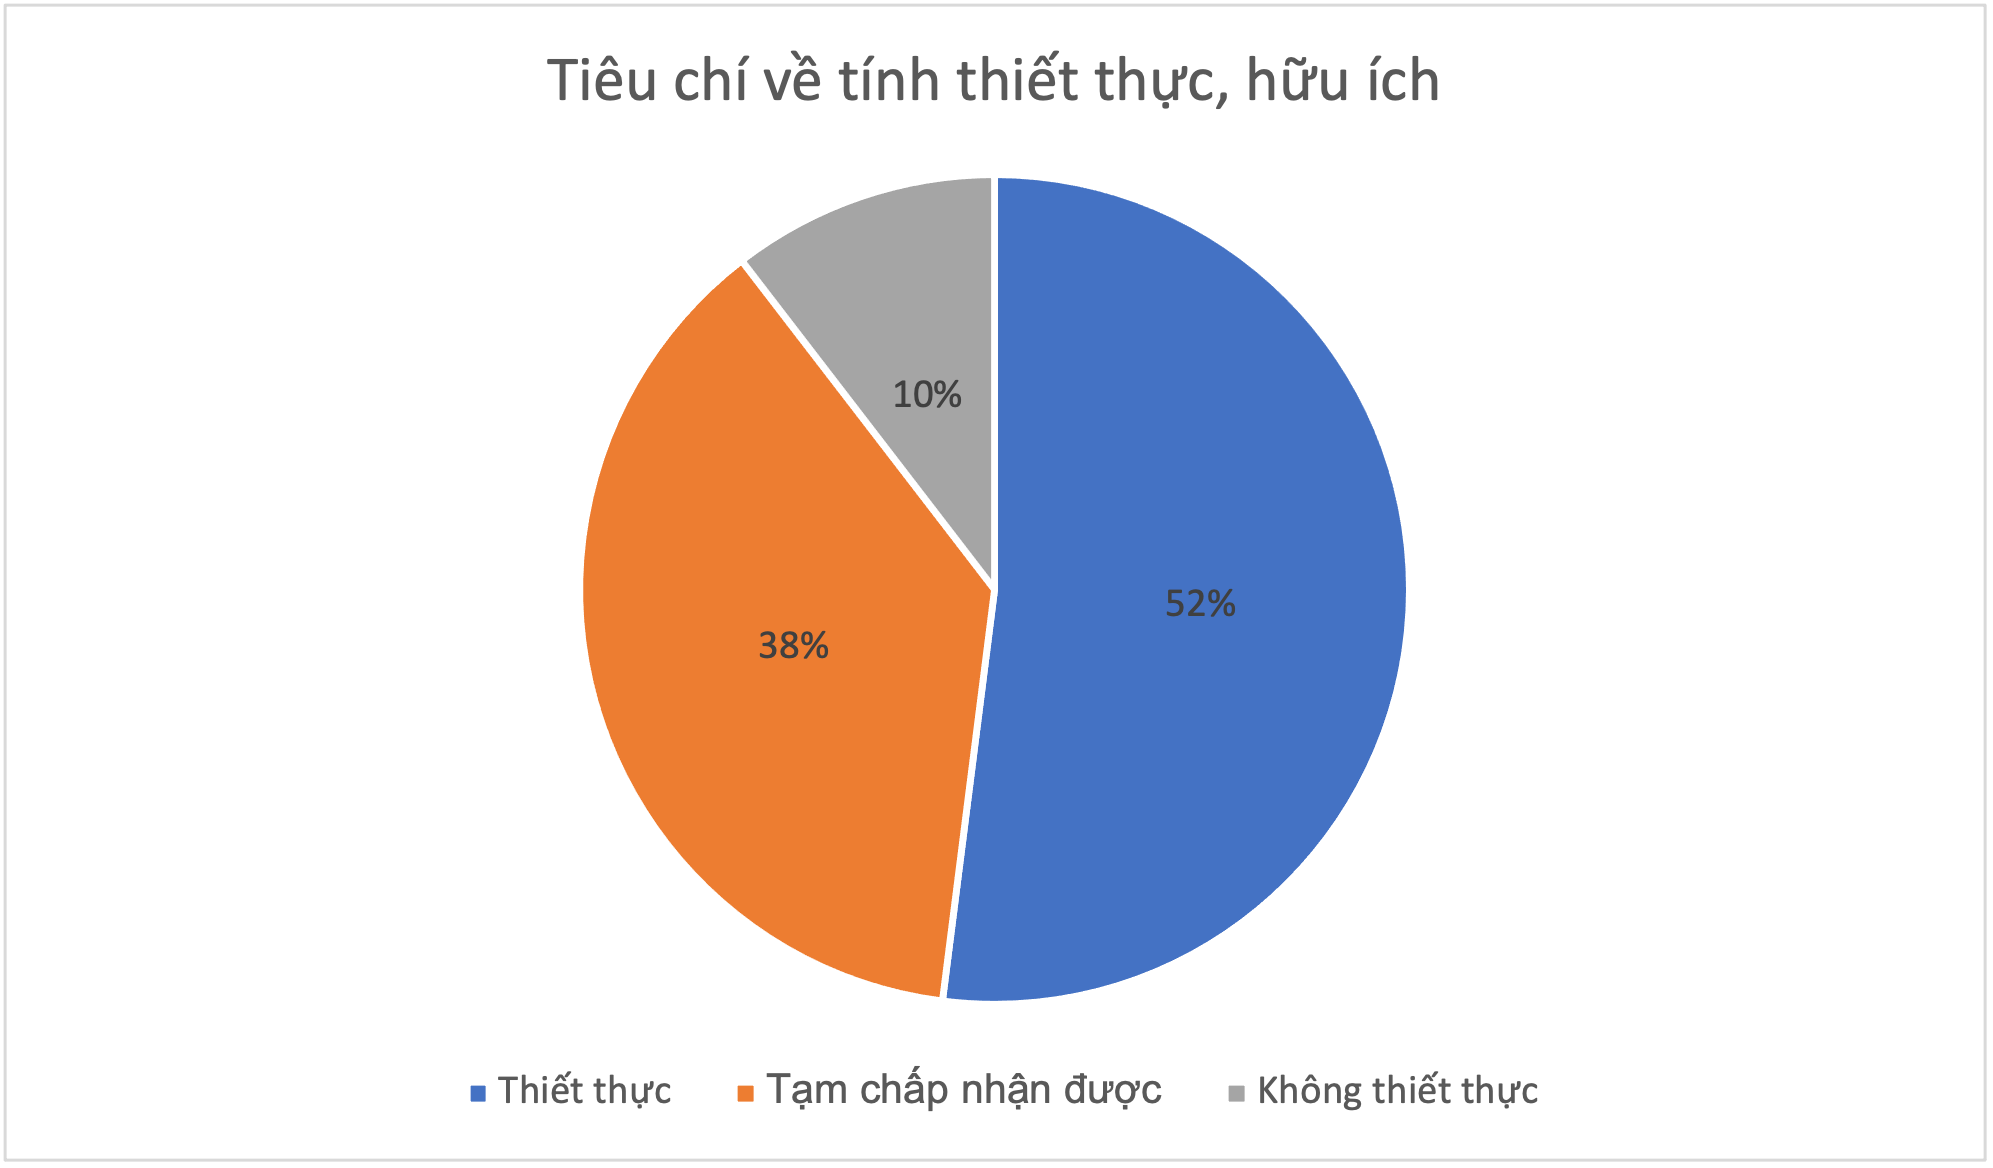
\includegraphics[scale=0.91]{thesis/chatbot/ketqua/img/tieuchi4.png}
    \caption{Kết quả đánh giá tiêu chí tính thiết thực, hữu ích}
    \label{fig:tieuchi4}
\end{figure}

\begin{figure}[ht!]
    \centering
    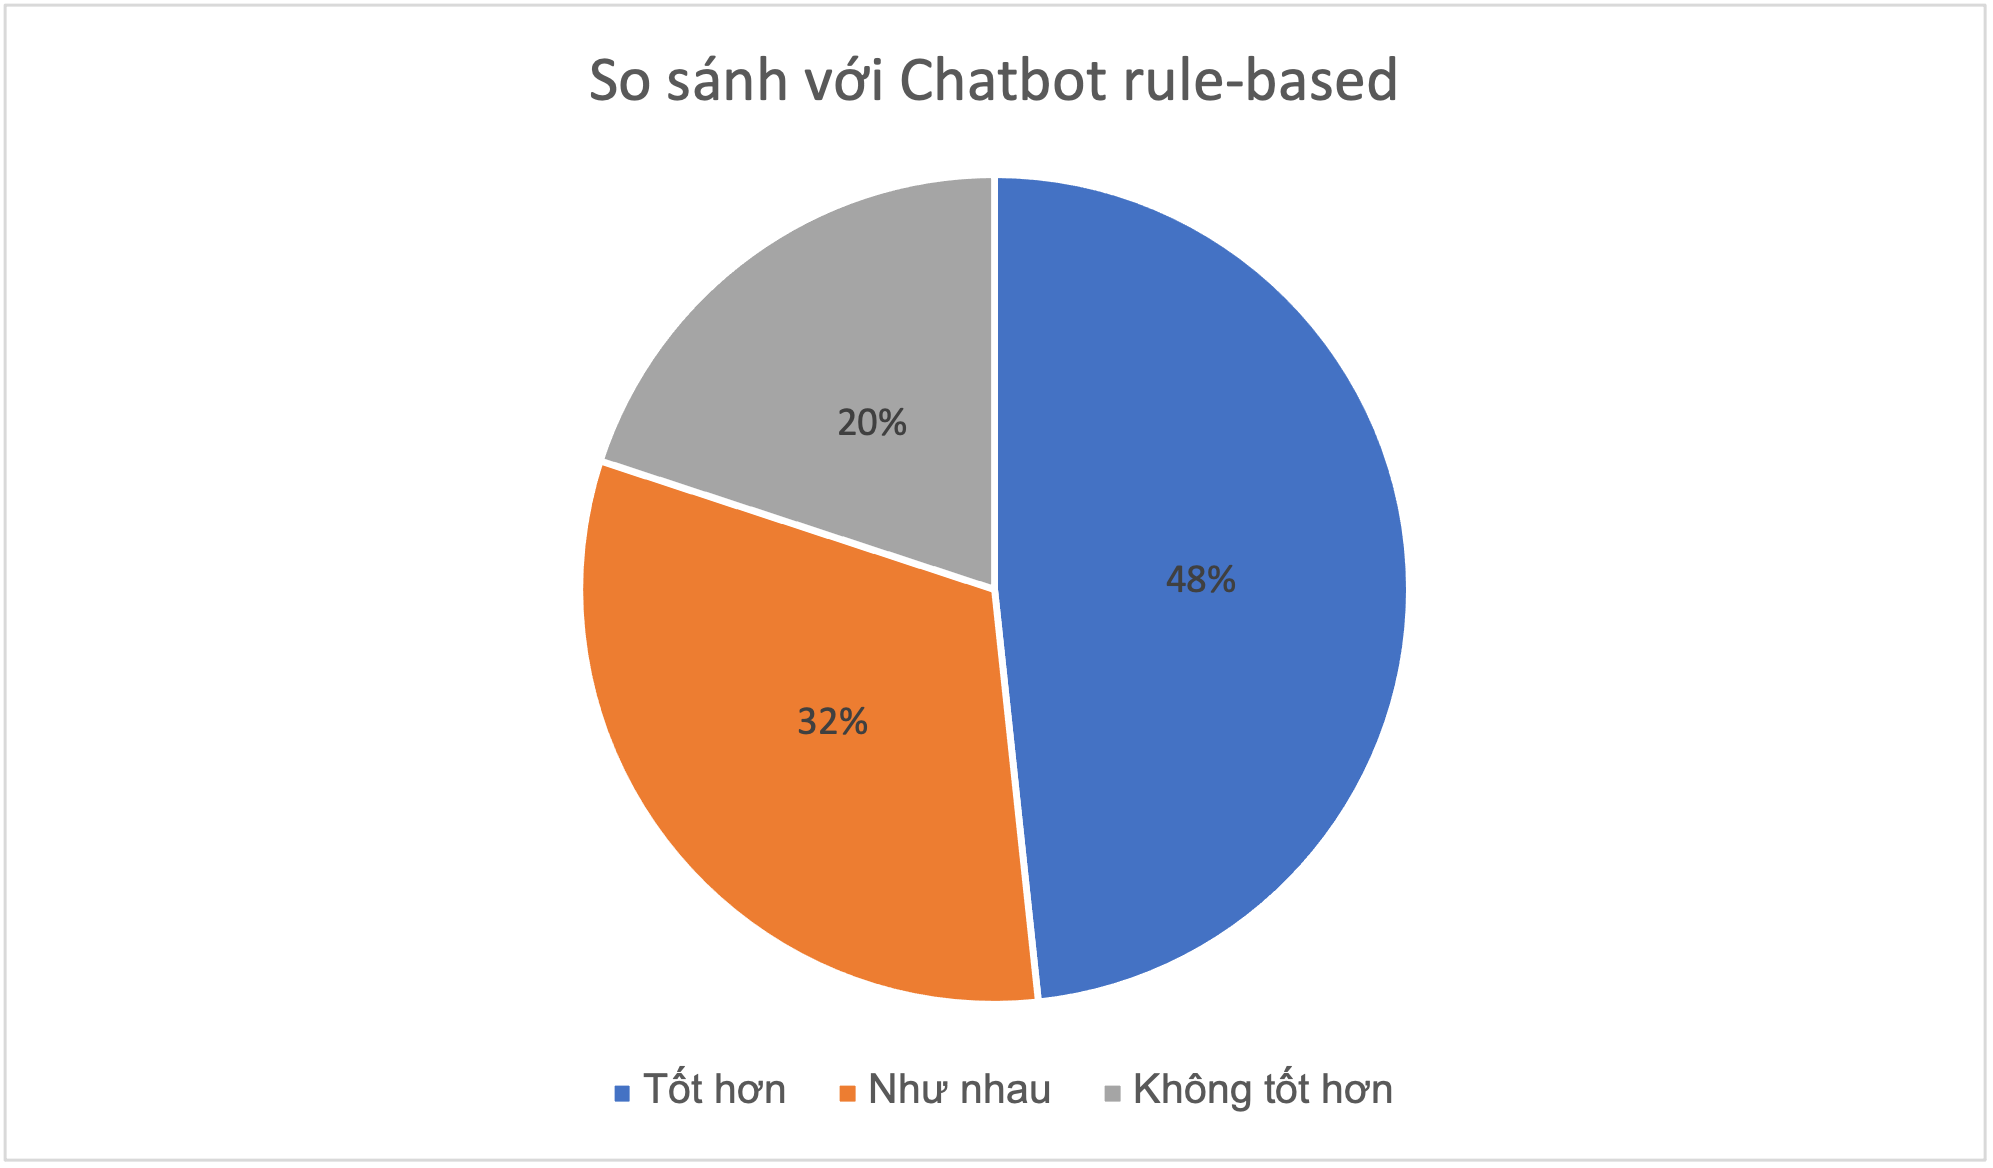
\includegraphics[scale=0.91]{thesis/chatbot/ketqua/img/tieuchi4_2.png}
    \caption{Kết quả so sánh với Chatbot rule-based}
    \label{fig:tieuchi42}
\end{figure}

\textbf{Nhận xét:}
Có 90\% nhận xét từ tạm chấp nhận được cho đến thiết thực. Trong đó
hơn 50\% là thiết thực. Chỉ có 10\% nhận xét là không thiết thực.
Nhận thấy việc gợi ý, cung cấp thông tin về sản phẩm giúp Chatbot
có thể thể hiện được khả năng hiểu vấn đề và khả năng cung cấp
thông tin có ích cho người dùng.

\subsubsection{So sánh với Chatbot rule-based}
Hình \ref{fig:tieuchi42} mô tả kết quả đánh giá của người dùng khi
so sánh tiêu chí tính thiết thực, hữu ích với Chatbot rule-based.

\textbf{Nhận xét:}
Có 80\% đánh giá là tốt hơn hoặc tương đương với Chatbot rule-based.
Có 20\% là không tốt hơn. Sau khi phân tích cụ thể các kết quả
đánh giá không tốt, nhận thấy Chatbot rule-based này sẽ liệt kê tất cả
thông tin của sản phẩm trong lượt đầu. Việc này thỏa mãn một số
người dùng tốt hơn Chatbot khi sử dụng học tăng cường.

\subsubsection{Tiêu chí về tính chính xác của các thông tin mà
tác nhân cung cấp}
Hình \ref{fig:tieuchi5} mô tả kết quả đánh giá của người dùng cho
tiêu chí tính chính xác của các thông tin mà tác nhân cung cấp.

\begin{figure}[ht!]
    \centering
    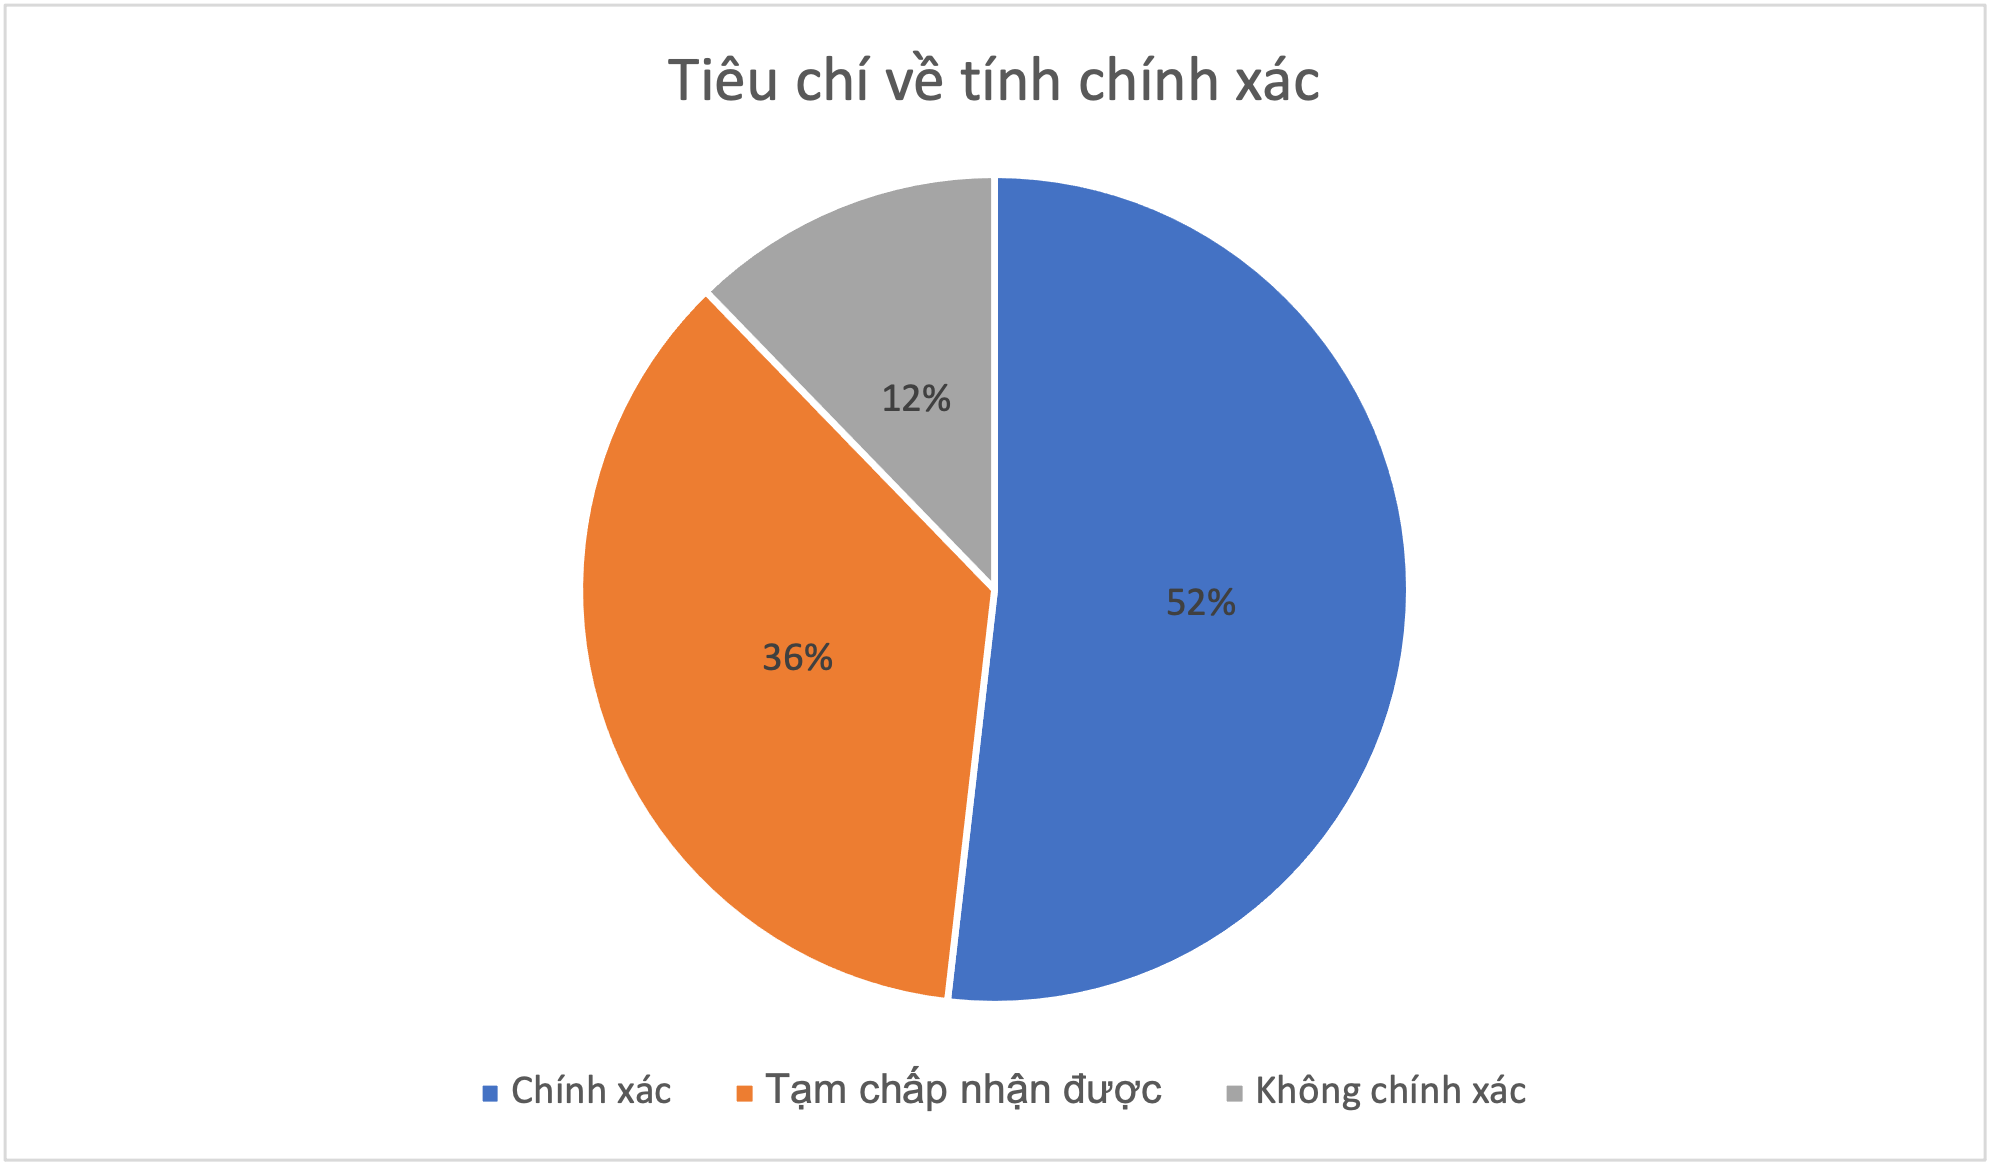
\includegraphics[scale=0.91]{thesis/chatbot/ketqua/img/tieuchi5.png}
    \caption{Kết quả đánh giá tiêu chí tính chính xác}
    \label{fig:tieuchi5}
\end{figure}

\textbf{Nhận xét:}
Có 90\% nhận xét từ tạm chấp nhận được cho đến chính xác. Trong đó
hơn 50\% là chính xác. Chỉ có 12\% nhận xét là không chính xác.
Hiện tại việc xác định thông tin người dùng thắc mắc là đúng hay
sai chỉ thực hiện thông qua phương pháp so trùng đơn giản nên việc
xác định này cũng còn khá hạn chế.

\subsubsection{Tiêu chí về mức độ đáp ứng nhu cầu tư vấn sản phẩm
nói chung}
Hình \ref{fig:tieuchi6} mô tả kết quả đánh giá của người dùng cho
tiêu chí về mức độ đáp ứng nhu cầu tư vấn sản phẩm nói chung.

\begin{figure}[ht!]
    \centering
    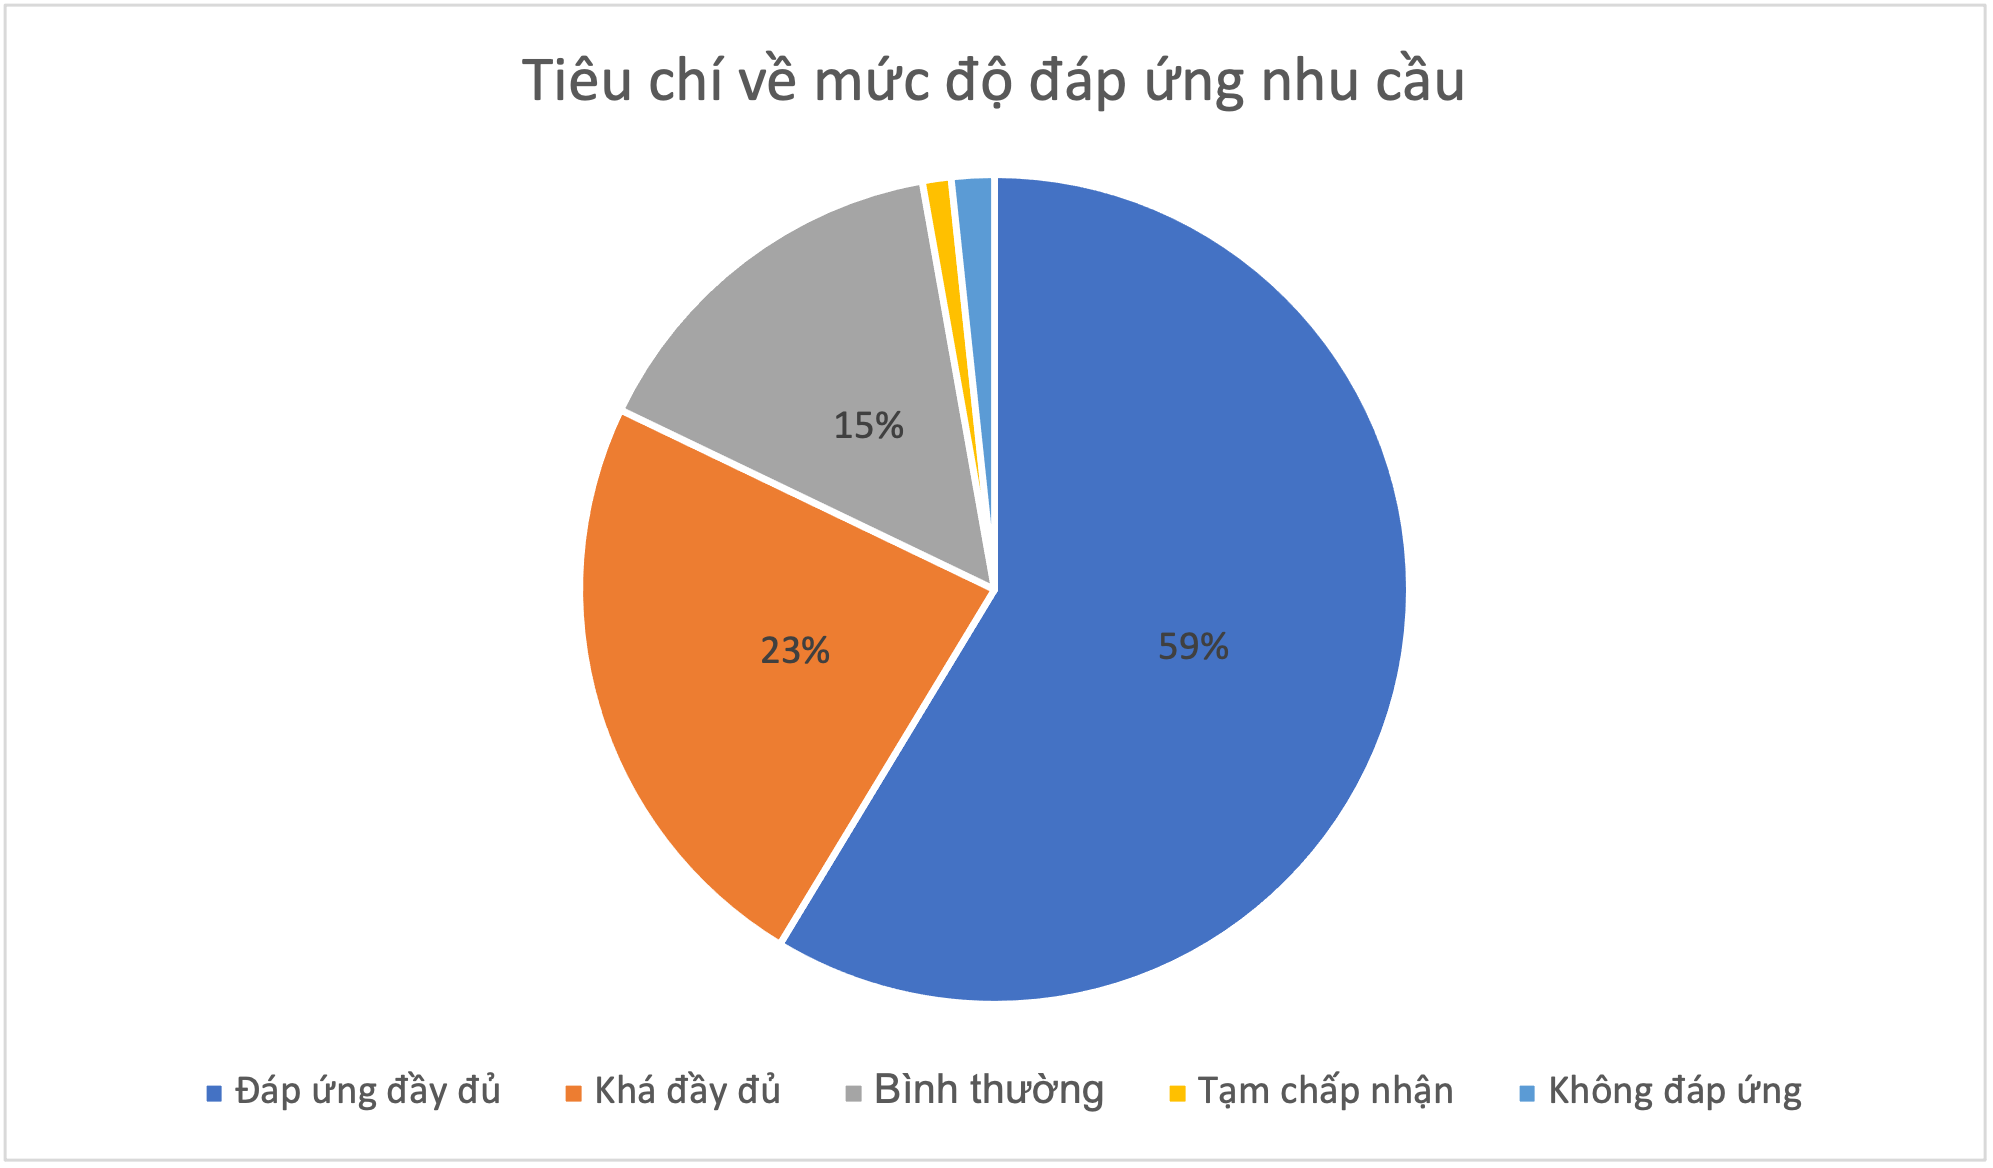
\includegraphics[scale=0.91]{thesis/chatbot/ketqua/img/tieuchi6.png}
    \caption{Kết quả đánh giá tiêu chí mức độ đáp ứng nhu cầu}
    \label{fig:tieuchi6}
\end{figure}

\begin{figure}[ht!]
    \centering
    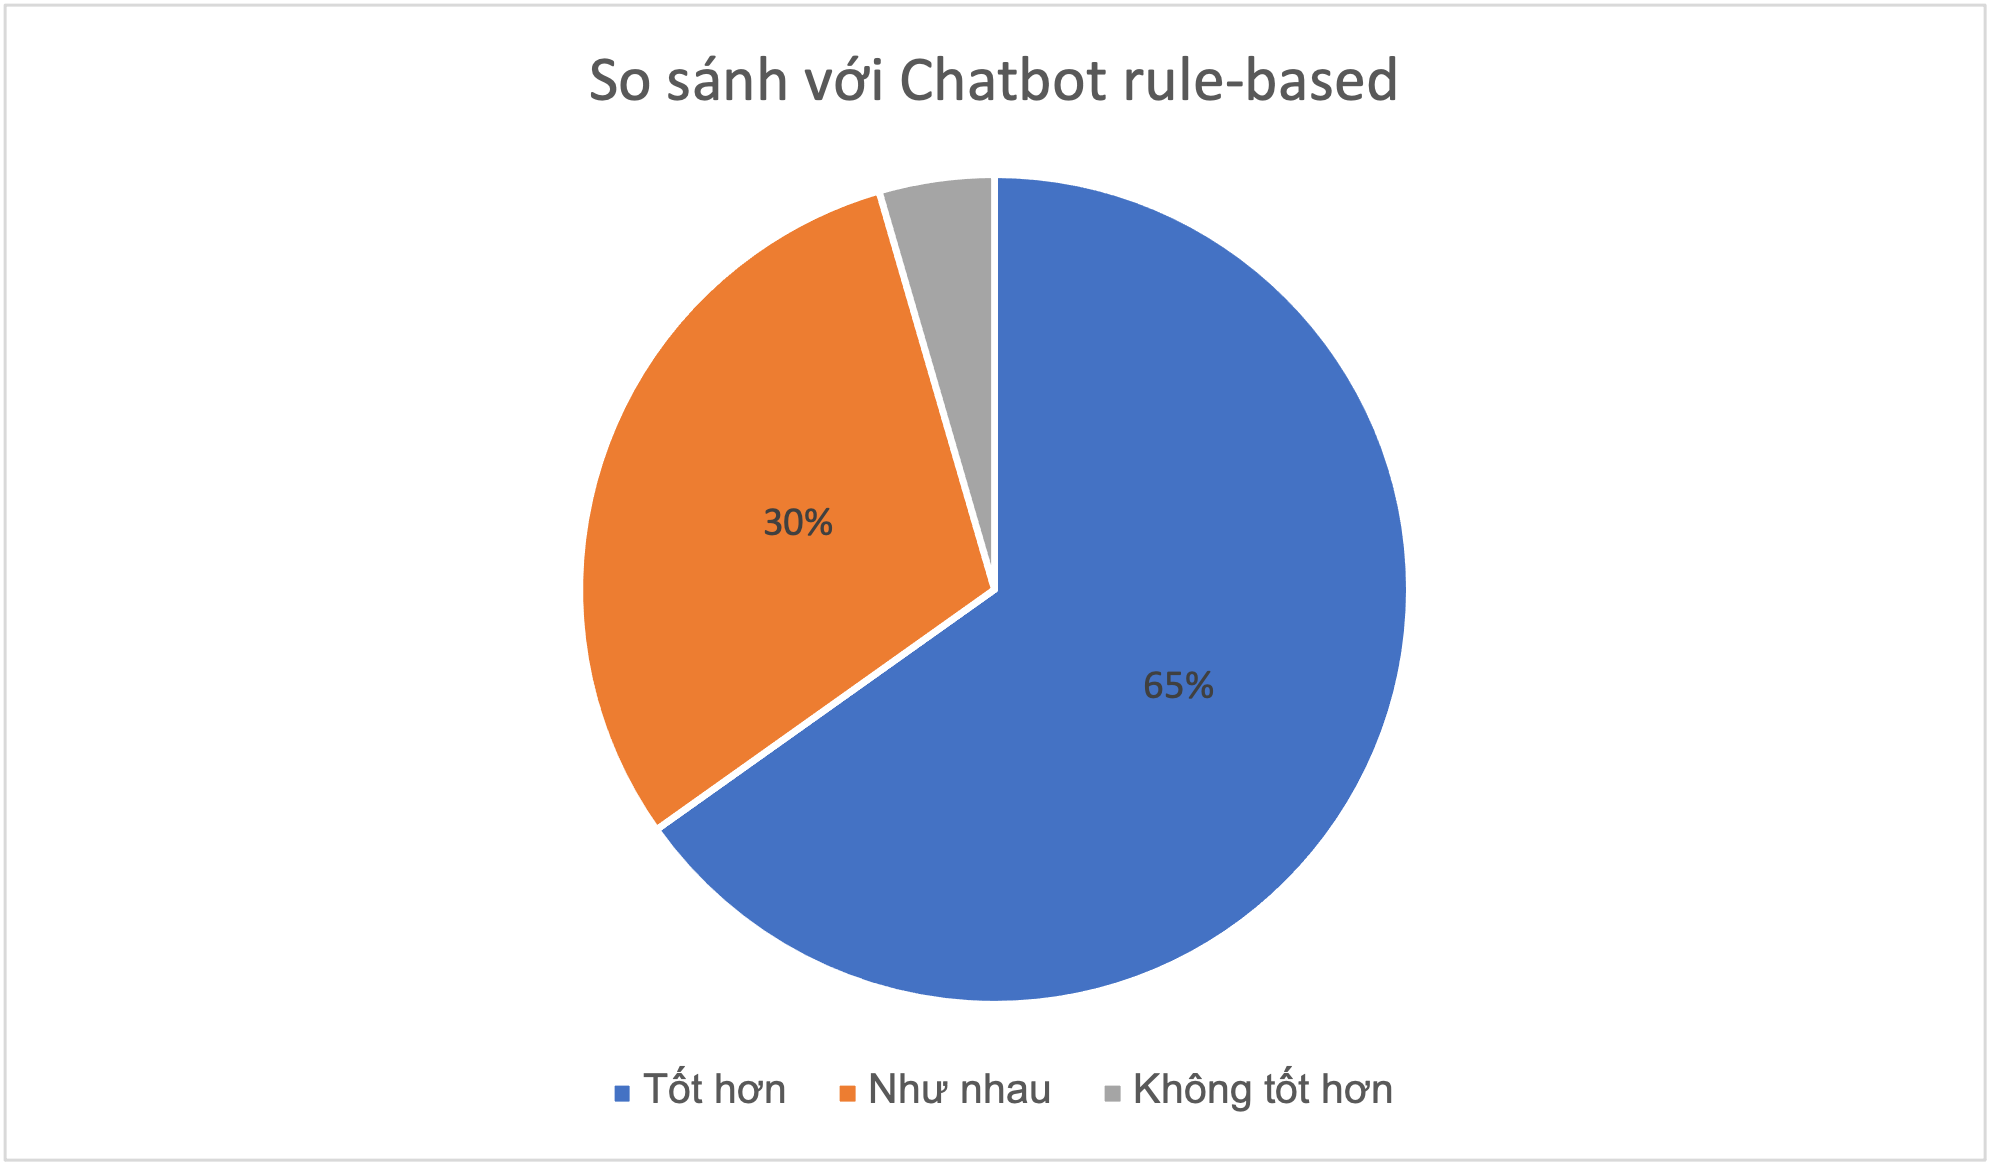
\includegraphics[scale=0.91]{thesis/chatbot/ketqua/img/tieuchi6_2.png}
    \caption{Kết quả so sánh với Chatbot rule-based}
    \label{fig:tieuchi62}
\end{figure}

\textbf{Nhận xét:}
Có 97\% nhận xét từ bình thường cho đến đáp ứng đầy đủ. Trong đó hơn
50\% là đáp ứng đầy đủ. Kết quả đánh giá như vậy là rất cao. Biểu thị
Chatbot được huấn luyện đáp ứng rất tốt các yêu cầu của người dùng.
Tuy nhiên, ta vẫn có 2\% nhận xét là không đáp ứng. Như đã đề cập về
những hạn chế ở những mục trước cũng như vấn đề về dữ liệu thực tế
chưa thực sự đầy đủ dẫn đến việc thông tin người dùng cần vẫn
chưa được cung cấp đầy đủ và chính xác.

\subsubsection{So sánh với Chatbot rule-based}
Hình \ref{fig:tieuchi62} mô tả kết quả đánh giá của người dùng khi
so sánh tiêu chí mức độ đáp ứng nhu cầu với Chatbot rule-based.

\textbf{Nhận xét:}
Có 95\% đánh giá là tốt hơn hoặc tương đương với Chatbot rule-based.
Chỉ có 5\% là không tốt hơn. Tương tự với nguyên nhân được đề cập ở
các tiêu chí trước, Chatbot rule-based này sẽ liệt kê tất cả thông tin
của sản phẩm trong lượt đầu. Việc này thỏa mãn một số người dùng tốt
hơn Chatbot khi sử dụng học tăng cường.

\subsubsection{Tiêu chí về mức độ giao tiếp tự nhiên trong suốt
cuộc hội thoại}
Hình \ref{fig:tieuchi7} mô tả kết quả đánh giá của người dùng cho
tiêu chí về mức độ giao tiếp tự nhiên trong suốt cuộc hội thoại.

\begin{figure}[ht!]
    \centering
    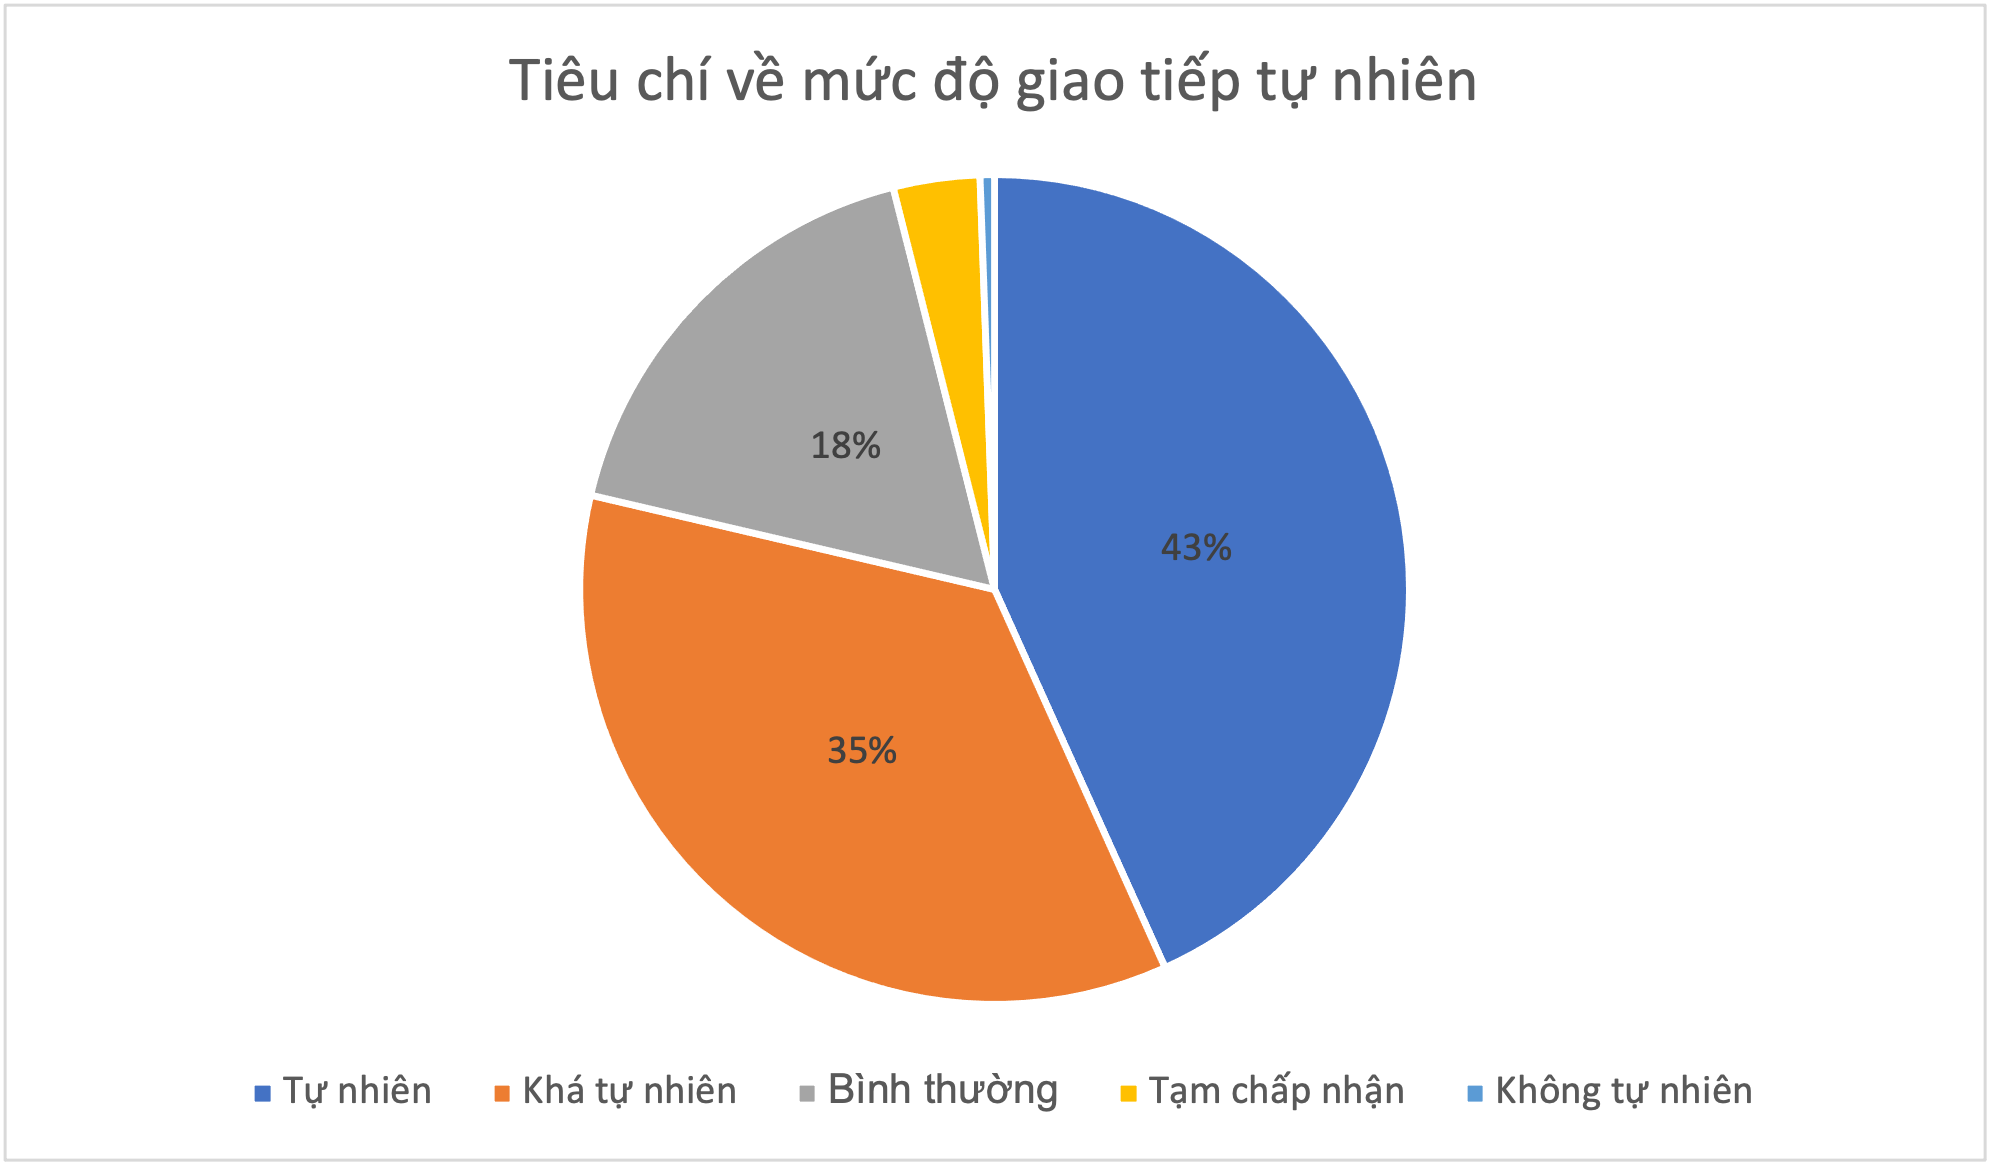
\includegraphics[scale=0.91]{thesis/chatbot/ketqua/img/tieuchi7.png}
    \caption{Kết quả đánh giá tiêu chí mức độ giao tiếp tự nhiên}
    \label{fig:tieuchi7}
\end{figure}

\textbf{Nhận xét:}
Có 96\% nhận xét từ bình thường cho đến tự nhiên. Trong đó gần 50\%
là tự nhiên. Chỉ có 1\% là không tự nhiên. Kết quả đánh giá như vậy
là rất cao. Biểu thị Chatbot được huấn luyện giao tiếp với người dùng
một cách tự nhiên phù hợp.

\subsubsection{So sánh với Chatbot rule-based}
Hình \ref{fig:tieuchi72} mô tả kết quả đánh giá của người dùng khi
so sánh tiêu chí mức độ giao tiếp tự nhiên với Chatbot rule-based.

\begin{figure}[ht!]
    \centering
    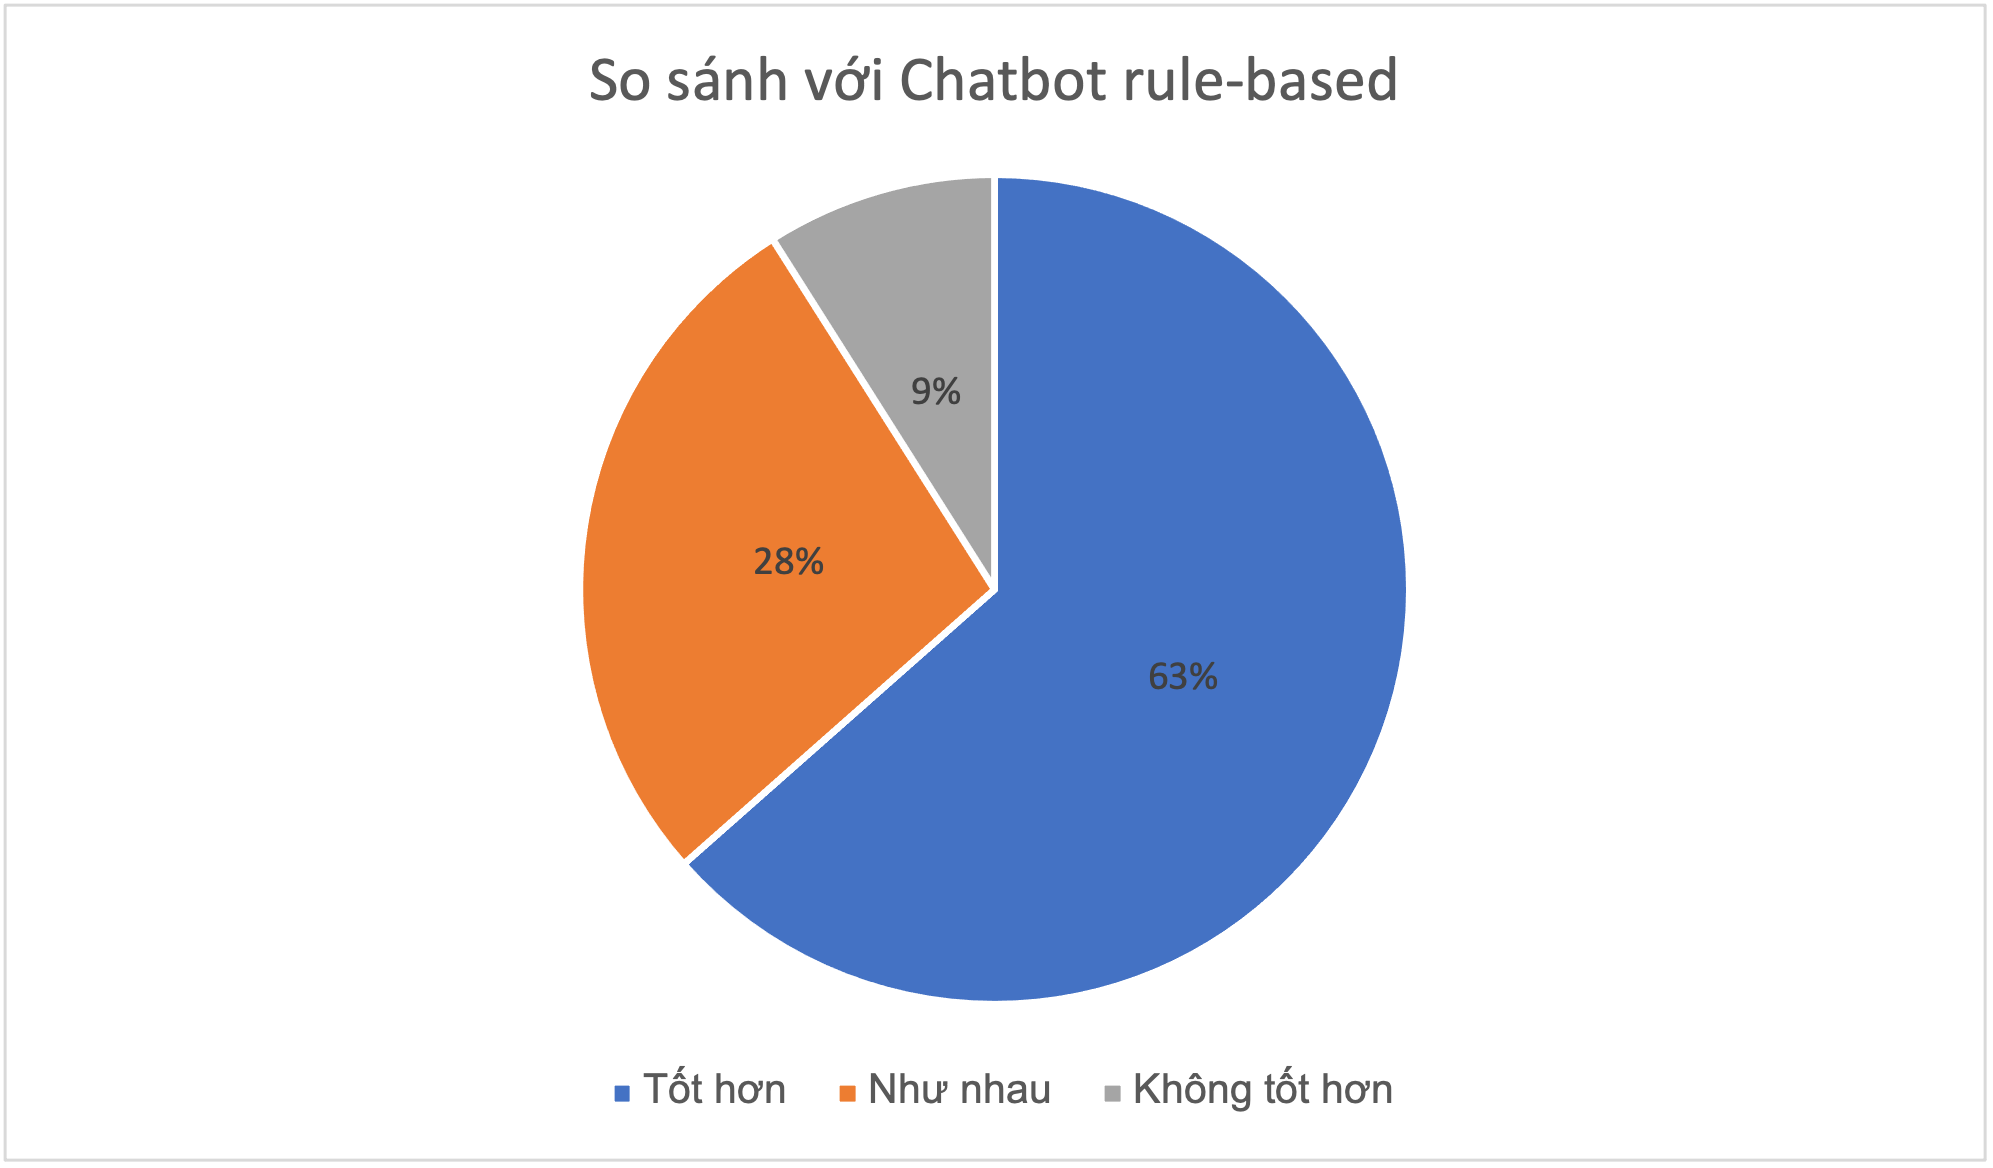
\includegraphics[scale=0.91]{thesis/chatbot/ketqua/img/tieuchi7_2.png}
    \caption{Kết quả so sánh với Chatbot rule-based}
    \label{fig:tieuchi72}
\end{figure}

\textbf{Nhận xét:}
Có hơn 90\% đánh giá là tốt hơn hoặc tương đương với Chatbot rule-based.
Chỉ có 9\% là không tốt hơn. Yếu tố tự nhiên được đánh giá tùy vào
cảm tính của người dùng. Một phần có thể do bộ sinh phản hồi
chưa được tốt.

\subsubsection{Đánh giá tổng quan của người dùng}
Hình \ref{fig:tieuchi8} mô tả kết quả đánh giá tổng quan của người dùng
trên thang đánh giá 5 sao.

\begin{figure}[ht!]
    \centering
    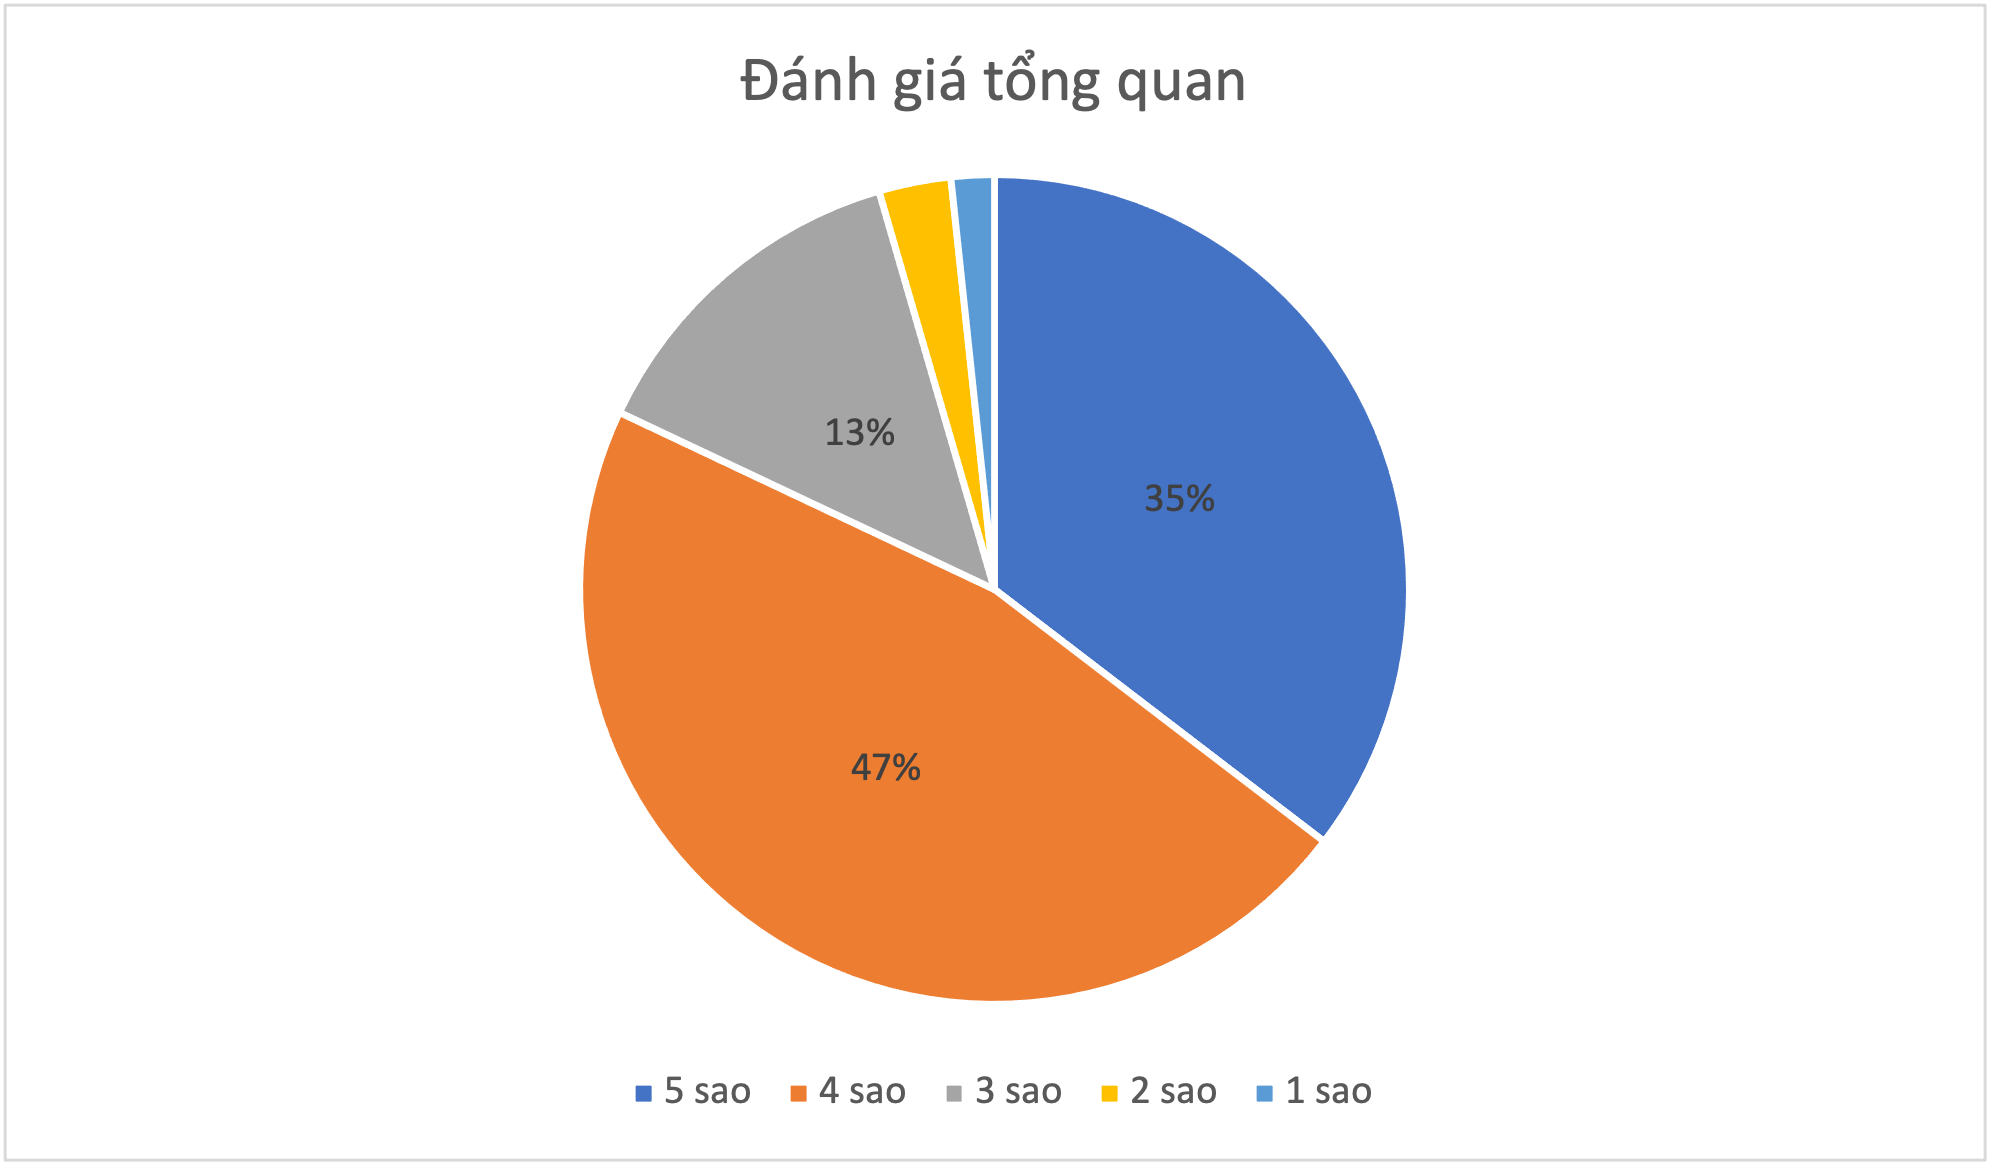
\includegraphics[scale=0.91]{thesis/chatbot/ketqua/img/tieuchi8.png}
    \caption{Kết quả đánh giá tổng quan của người dùng}
    \label{fig:tieuchi8}
\end{figure}

\textbf{Nhận xét:}
Kết quả cho thấy có 95\% người dùng đánh giá từ 3 sao trở lên.
Xét trên thang điểm 5 sao, Chatbot đạt 4.1 sao.

\section{Kiểm thử ứng dụng Chatbot}
Kiểm thử hệ thống thuộc loại kiểm thử hộp đen (black box). Kiểm thử
hệ thống là kiểm tra được thực hiện trên một hệ thống tích hợp
hoàn chỉnh để đánh giá sự tuân thủ của hệ thống với các yêu cầu đã
chỉ định của nó. Nội dung kiểm thử và tiêu chí đánh giá được
mô tả cụ thể sau đây.

\subsection{Kiểm thử giao diện}
Nội dung kiểm thử được mô tả cụ thể ở bảng \ref{tab:uitest}.

\begin{table}[!ht]
\caption{Đặc tả kiểm thử giao diện Chatbot}
\label{tab:uitest}
\centering
\begin{tabular}{|C{0.8cm}|L{3.2cm}|L{3.2cm}|L{3.6cm}|C{1.8cm}|}
\hline
\textbf{STT} &
\centering\textbf{Chức năng} &
\centering\textbf{Nội dung kiểm thử} &
\centering\textbf{Kết quả mong đợi} &
\textbf{Kết quả kiểm thử} \\ % inserts table %heading
\hline
1 &
Giao diện Chatbot với các nút bấm chức năng, ô lựa chọn, khung
hội thoại và toàn bộ tin nhắn của người dùng và tác nhân cho tới
thời điểm hiện tại &
Bước 1: Truy cập vào ứng dụng Chatbot.
Bước 2: Thực hiện thao tác trên các nút bấm chức năng. &
Giao diện Chatbot hiển thị đầy đủ các nút bấm, ô lựa chọn, khung
hội thoại và toàn bộ tin nhắn của người dùng và tác nhân cho tới
thời điểm hiện tại, Kết quả minh họa như hình \ref{fig:testtool} &
PASS \\
\hline
2 &
Giao diện Chatbot với kích thước trên các thiết bị có độ
phân giải và kích thước khác nhau &
Bước 1: Truy cập vào ứng dụng Chatbot với các
trình duyệt khác nhau.
Bước 2: Thu nhỏ hoặc phóng lớn cửa sổ. &
Giao diện Chatbot giữ nguyên kích thước trên các thiết bị có độ
phân giải và kích thước khác nhau, không bị khuất, bị mất nội dung &
PASS \\
\hline
3 &
Các hiệu ứng hành động trên giao diện Chatbot &
Bước 1: Truy cập vào ứng dụng Chatbot.
Bước 2: Thực hiện thao tác trên ứng dụng, quan sát các thay đổi
trên giao diện. &
Các hiệu ứng hành động trên giao diện Chatbot hiển thị mượt mà,
không gặp hiện tượng giật, đứng khi sử dụng &
PASS \\
\hline
\end{tabular}
\end{table}

\begin{figure}[ht!]
    \centering
    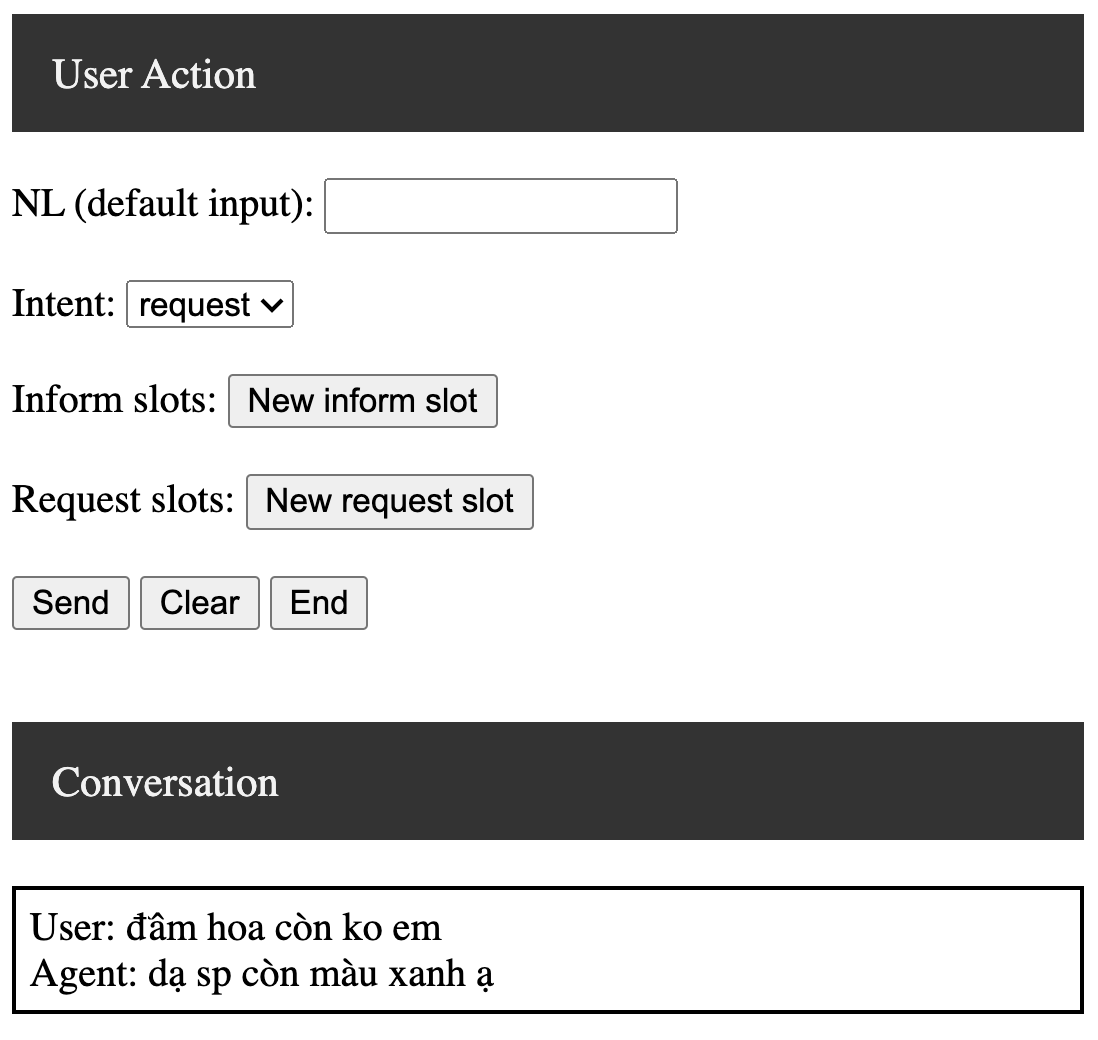
\includegraphics[scale=0.6]{thesis/chatbot/ketqua/img/test_tool.png}
    \caption{Giao diện của Chatbot}
    \label{fig:testtool}
\end{figure}

\subsection{Kiểm thử chức năng}
Nội dung kiểm thử được mô tả cụ thể ở bảng \ref{tab:functiontest}.

\begin{table}[!ht]
\caption{Đặc tả kiểm thử chức năng Chatbot}
\centering
\begin{tabular}{|C{0.8cm}|L{2cm}|L{4.4cm}|L{3.6cm}|C{1.8cm}|}
\hline
\textbf{STT} &
\centering\textbf{Chức năng} &
\centering\textbf{Nội dung kiểm thử} &
\centering\textbf{Kết quả mong đợi} &
\textbf{Kết quả kiểm thử} \\ % inserts table %heading
\hline
1 &
Gửi hành động người dùng &
Bước 1: Nhập câu thoại hoặc lựa chọn hành động thông qua các ô lựa chọn.
Bước 2: Gửi hành động. &
Chatbot nhận được hành động của người dùng, không sai lệch, thiếu thông tin &
PASS \\
\hline
2 &
Xóa hành động người dùng &
Bước 1: Nhập câu thoại hoặc lựa chọn hành động thông qua các ô lựa chọn.
Bước 2: Xóa hành động. &
Chatbot xóa hành động đang nhập hiện tại của người dùng.
Trạng thái hội thoại không thay đổi &
PASS \\
\hline
3 &
Phản hồi người dùng &
Bước 1: Nhập câu thoại hoặc lựa chọn hành động thông qua các ô lựa chọn.
Bước 2: Gửi hành động. &
Chatbot có phản hồi với mỗi tin nhắn của người dùng và hiển thị câu
phản hồi trên khung hội thoại &
PASS \\
\hline
4 &
Kết thúc hội thoại &
Bước 1: Nhập câu thoại hoặc lựa chọn hành động thông qua các ô lựa chọn.
Bước 2: Gửi hành động.
Bước 3: Nhấn nút kết thúc hội thoại. &
Chatbot xóa toàn bộ nội dung hội thoại, đồng thời thiết lập lại
trạng thái hội thoại &
PASS \\
\hline
\end{tabular}
\label{tab:functiontest}
\end{table}

% \subsection{Kiểm thử đơn vị}

% \subsubsection{Bộ truy vấn cơ sở dữ liệu}

% \subsubsection{Bộ xử lý phản hồi người dùng}

% \subsubsection{Bộ quản lý trạng thái hội thoại}

% \subsubsection{Bộ sinh phản hồi}

% \subsubsection{Bộ sinh câu phản hồi}
